% ============================================================
%  FedQPSO: IEEE Conference Paper
%  Author: Divyansh Teja Edla
%  Matrusri Engineering College, Hyderabad, India
% ============================================================
\documentclass[conference]{IEEEtran}
\IEEEoverridecommandlockouts

\usepackage{cite}
\usepackage{amsmath,amssymb,amsfonts}
\usepackage{algorithmic}
\usepackage{algorithm}
\usepackage{graphicx}
\usepackage{textcomp}
\usepackage{xcolor}
\usepackage{booktabs}
\usepackage{multirow}
\usepackage{array}
\usepackage{url}
\usepackage{hyperref}

\graphicspath{{figs/}}

\def\BibTeX{{\rm B\kern-.05em{\sc i\kern-.025em b}\kern-.08em
    T\kern-.1667em\lower.7ex\hbox{E}\kern-.125emX}}

% ============================================================
\begin{document}
% ============================================================

\title{FedQPSO: Layer-by-Layer Quantum Particle Swarm Optimization for
Equitable Federated Brain Tumor Classification Under Non-IID Data
\thanks{This work was supported by the Department of Computer Science \&
Engineering, Matrusri Engineering College, Hyderabad, India.}}

\author{%
\IEEEauthorblockN{Divyansh Teja Edla}
\IEEEauthorblockA{\textit{Dept.\ of Computer Science \& Engineering}\\
\textit{Matrusri Engineering College}\\
Hyderabad, India\\
divyanshteja.edla@gmail.com}
}

\maketitle

% ============================================================
\begin{abstract}
Federated Learning (FL) enables privacy-preserving collaborative training
across medical institutions without sharing raw patient data, yet standard
Federated Averaging (FedAvg) produces global accuracy that conceals severe
per-institution performance disparities. We propose \textbf{FedQPSO}, a
server-side aggregation algorithm that applies layer-by-layer Quantum Particle
Swarm Optimization (QPSO) with combined cross-client validation-loss fitness
evaluation — creating an implicit fairness constraint without any explicit
fairness regularizer. Evaluated on four-class brain tumor MRI classification
across three heterogeneous simulated clinical sites under two conditions —
natural heterogeneity (Setup~1) and moderate label skew 70/10/10/10
(Setup~2) — FedQPSO achieves the best client fairness in both conditions.
Under natural heterogeneity, FedQPSO reduces the inter-client performance
standard deviation to 1.56\% versus 2.27\% (FedProx) and 5.28\% (FedAvg),
and shrinks the max-min accuracy gap by 81\%. Under label skew, FedQPSO is
the \emph{only} method maintaining clinically useful accuracy ($\geq$80\%) at
the weakest client. FedQPSO achieves the highest Glioma recall in both setups
(0.9593; 0.8914), the most stable accuracy trajectories (maximum per-round drop:
3.38\,pp vs.\ 14.78\,pp for FedAvg), and is the only method statistically
significantly outperforming FedAvg under natural heterogeneity ($p=0.000882$,
Cohen's $d=0.35$). Effect size grows from $d=0.35$ to $d=1.26$ as
heterogeneity increases, confirming FedQPSO is most advantageous precisely
when conditions are most challenging.
\end{abstract}

\begin{IEEEkeywords}
Federated learning, quantum particle swarm optimization, FedQPSO, brain tumor
classification, non-IID data, client fairness, medical imaging, MRI
\end{IEEEkeywords}

% ============================================================
\section{Introduction}
\label{sec:intro}
% ============================================================

Brain tumors are among the most lethal cancers, with a five-year survival
rate under 36\% for malignant cases \cite{ostrom2021}. Accurate
classification of tumor type from Magnetic Resonance Imaging (MRI) is
fundamental to treatment planning: gliomas demand immediate surgical
evaluation, meningiomas are typically benign, pituitary adenomas are often
managed pharmacologically, and correctly identifying tumor absence prevents
unnecessary interventions. Deep learning models trained on large, diverse
datasets can assist radiologists with near-expert accuracy \cite{sultan2019}.

The central barrier to assembling such datasets is \emph{data privacy}.
Medical imaging data is among the most strictly regulated personal data
globally: HIPAA in the United States \cite{hipaa}, GDPR in the European
Union, and comparable regulations across Asia impose strict prohibitions on
sharing raw patient records. Traditional centralized training constitutes a
direct privacy violation.

\textbf{Federated Learning (FL)} \cite{mcmahan2017} resolves this by
decoupling training from data centralization: a central server broadcasts a
global model, each hospital trains locally on private data, and only weight
updates --- never raw images --- are returned. The server aggregates updates
and repeats for multiple communication rounds.

However, real-world medical federations exhibit \textbf{Non-IID} data.
Hospitals differ in scanner equipment, patient demographics, and class
distributions. Standard FedAvg \cite{mcmahan2017} computes a
dataset-size-weighted average of client weights. Under Non-IID conditions,
this is dominated by large clients, causing the global model to
systematically underperform for smaller or data-imbalanced institutions
\cite{zhao2018}. A model achieving 95\% global accuracy but 60\% accuracy
at one hospital is clinically \emph{inequitable}.

FedProx \cite{li2020fedprox} partially addresses this by penalizing client
drift via a proximal term, but does not fundamentally redistribute influence
from large to small clients. SCAFFOLD \cite{karimireddy2020scaffold} reduces
drift via control variates, and personalized FL \cite{kulkarni2020pfl} allows
local adaptation, but none explicitly optimize for cross-client equity during
aggregation.

In prior work \cite{edla2025mnist}, we demonstrated that Quantum Particle
Swarm Optimization (QPSO) \cite{sun2004qpso} applied layer-by-layer as a
federated aggregation strategy outperforms FedAvg on IID MNIST data. The
key mechanism: candidate weight configurations are evaluated against a
\emph{combined cross-client validation set} before being committed, making
the optimization naturally fairness-aware.

This paper presents \textbf{FedQPSO}, the first application of layer-by-layer
QPSO aggregation to Non-IID federated medical image classification, with
a four-phase experimental study on brain tumor MRI.

\textbf{Key contributions:}
\begin{enumerate}
    \item \textbf{FedQPSO algorithm:} Novel federated aggregation performing
    layer-by-layer QPSO with validation-loss fitness evaluation, functioning
    as an implicit fairness mechanism requiring no explicit fairness objective.

    \item \textbf{Fairness discovery:} Formal demonstration that combined
    validation-set fitness evaluation reduces the max-min per-client gap by
    72--81\% vs.\ FedAvg and 45--56\% vs.\ FedProx.

    \item \textbf{Clinical equity:} FedQPSO is the \emph{only} method
    maintaining clinically meaningful accuracy ($\geq$80\%) at the weakest
    client under label skew, with the highest Glioma recall in both setups.

    \item \textbf{Stability:} Most stable accuracy trajectory across both
    conditions (max crash 3.38\,pp vs.\ 14.78\,pp for FedAvg).

    \item \textbf{Heterogeneity scaling:} FedQPSO's statistical advantage
    grows with heterogeneity severity (Cohen's $d$: $0.35 \to 1.26$).
\end{enumerate}

% ============================================================
\section{Related Work}
\label{sec:related}
% ============================================================

\subsection{Federated Learning for Medical Imaging}
McMahan et al.\ \cite{mcmahan2017} introduced FedAvg in 2017. Sheller et al.\
\cite{sheller2018} pioneered its application to brain tumor \emph{segmentation}
on the BraTS dataset, showing that FL can approach centralized performance.
Rieke et al.\ \cite{rieke2020} surveyed FL in healthcare, identifying Non-IID
data as the central unsolved challenge. Our work extends Sheller et al.'s
paradigm to tumor \emph{classification} with a fairness-focused aggregation
strategy.

\subsection{Non-IID Data in Federated Learning}
Li et al.\ \cite{li2020fedprox} proposed FedProx, adding proximal term
$(\mu/2)\|w - w_{\text{global}}\|^2$ to the client loss to limit drift.
Karimireddy et al.\ \cite{karimireddy2020scaffold} introduced SCAFFOLD using
control variates to reduce drift variance. Zhao et al.\ \cite{zhao2018}
confirmed label skew as the most challenging heterogeneity form. These
approaches modify \emph{client-side} training; FedQPSO redesigns
\emph{server-side aggregation} to be fitness-guided and fairness-aware.

\subsection{PSO and QPSO in Machine Learning}
Classical PSO \cite{kennedy1995} has been applied to neural architecture
search and hyperparameter optimization. FedPSO \cite{fedpso2021} uses
classical PSO for global FL model updates, transmitting score values rather
than tensors to reduce communication overhead. Sun et al.\ \cite{sun2004qpso}
introduced QPSO with theoretically proven global search capability via a
quantum potential well model. Our prior work \cite{edla2025mnist} first applied
layerwise QPSO to FL aggregation on IID MNIST (achieving 81.5\% vs.\ FedAvg's
41.2\%). The present paper extends this to Non-IID medical imaging with formal
fairness analysis.

% ============================================================
\section{System Model and Problem Formulation}
\label{sec:problem}
% ============================================================

Let $\mathcal{K} = \{1, 2, \ldots, K\}$ be a set of $K$ clients, each
holding a private dataset $\mathcal{D}_k$ with $n_k$ labeled samples, and
$N = \sum_k n_k$. The global FL objective is:
\begin{equation}
    \min_{w}\; F(w) = \sum_{k=1}^{K} \frac{n_k}{N}\, F_k(w),
    \label{eq:fl_objective}
\end{equation}
where $F_k(w) = \mathbb{E}_{(x,y)\sim\mathcal{D}_k}[\ell(w;\,x,y)]$.
Under Non-IID conditions, minimizing~\eqref{eq:fl_objective} produces biased
solutions that minimize average loss while leaving minority clients poorly
served.

We additionally pursue a \textbf{client fairness objective}:
\begin{equation}
    \min_{w}\; \sigma^2\!\left(F_1(w), F_2(w), \ldots, F_K(w)\right).
    \label{eq:fairness_objective}
\end{equation}
Both objectives can be simultaneously pursued if server-side aggregation
evaluates candidate weights against a \emph{balanced cross-client validation
set}, penalizing solutions that fail any institution.

% ============================================================
\section{Methodology}
\label{sec:method}
% ============================================================

\subsection{FedAvg (Baseline)}
Standard Federated Averaging \cite{mcmahan2017} aggregates client weights as
a dataset-size-weighted mean:
\begin{equation}
    w^{(r+1)} = \sum_{k=1}^{K} \frac{n_k}{N}\, w_k^{(r)},
    \label{eq:fedavg}
\end{equation}
where $w_k^{(r)}$ are locally-trained weights at round $r$. Under Non-IID
conditions, this weighted average is dominated by large clients, systematically
marginalizing smaller institutions.

\subsection{FedProx (Regularized Baseline)}
FedProx \cite{li2020fedprox} modifies client-side training with a proximal
regularization term:
\begin{equation}
    \mathcal{L}_{\text{FedProx}}(w_k) = \mathcal{L}_k(w_k)
    + \frac{\mu}{2}\,\|w_k - w_{\text{global}}\|^2,
    \label{eq:fedprox}
\end{equation}
with $\mu = 0.01$. Server-side aggregation remains identical to FedAvg.
The proximal term constrains all clients equally; it does not redistribute
influence from large to small clients.

\subsection{FedQPSO: Proposed Algorithm}

\subsubsection{QPSO Background}
QPSO \cite{sun2004qpso} treats each candidate solution as a particle in a
quantum potential well. Particle $i$ has position $x_i$, personal best
$\mathbf{pbest}_i$, and the swarm tracks global best $\mathbf{gbest}$. The
quantum-inspired update is:
\begin{align}
    \phi &\sim \mathcal{U}(0,1), \quad
    p_i = \phi\,\mathbf{pbest}_i + (1-\phi)\,\mathbf{gbest},
    \label{eq:attractor}\\
    \mathbf{mbest} &= \frac{1}{K}\sum_{k=1}^{K}\mathbf{pbest}_k,
    \label{eq:mbest}\\
    x_i^{(t+1)} &= p_i \pm \beta\,|{\mathbf{mbest}} - x_i^{(t)}|
    \cdot \ln\!\left(\frac{1}{u}\right), \quad u \sim \mathcal{U}(\varepsilon,1),
    \label{eq:qpso_update}
\end{align}
where the sign ($\pm$) is chosen uniformly at random and $\beta$ is the
contraction-expansion coefficient. The logarithmic distribution enables
quantum tunneling, allowing particles to escape local optima.

\subsubsection{Layer-by-Layer Federated Aggregation}
At each communication round $r$, after all clients complete local training,
the FedQPSO server executes Algorithm~\ref{alg:fedqpso}. The \emph{critical
design choice} is the layer-by-layer decomposition: optimizing all 120K
parameters simultaneously (as in naive QPSO) is equivalent to noise injection;
solving per-layer subproblems with fitness feedback is a genuine optimization
procedure.

\begin{algorithm}
\caption{FedQPSO server-side aggregation (round $r$)}
\label{alg:fedqpso}
\begin{algorithmic}[1]
\REQUIRE Client weight dicts $\{w_k\}_{k=1}^K$; combined val set
$\mathcal{V} = \bigcup_k \mathcal{V}_k$; $\beta$, iterations $T$
\STATE Compute FedAvg baseline $\bar{w}$ (covers BatchNorm running stats)
\FOR{each trainable layer $\ell = 1,\ldots,L$}
    \STATE $x_k \leftarrow w_k[\ell]$ for all $k$ \hfill \COMMENT{particles}
    \STATE Evaluate $\mathrm{fit}(x_k) \leftarrow \mathcal{L}(\bar{w}[x_k \to \ell],\;\mathcal{V})$
    \STATE $\mathbf{pbest}_k \leftarrow x_k$;\quad $\mathbf{gbest} \leftarrow \arg\min_k \mathrm{fit}(x_k)$
    \FOR{$t = 1$ to $T$}
        \STATE Compute $\mathbf{mbest}$ via \eqref{eq:mbest}
        \FOR{each particle $k$}
            \STATE Compute $p_k$ via \eqref{eq:attractor}; sample $u,\phi$; choose $\pm$
            \STATE $x_k^{(t+1)} \leftarrow p_k \pm \beta\,|\mathbf{mbest}-x_k^{(t)}|\cdot\ln(1/u)$
            \STATE Evaluate $\mathrm{fit}(x_k^{(t+1)})$
            \IF{$\mathrm{fit}(x_k^{(t+1)}) < \mathrm{fit}(\mathbf{pbest}_k)$}
                \STATE $\mathbf{pbest}_k \leftarrow x_k^{(t+1)}$
            \ENDIF
            \IF{$\mathrm{fit}(x_k^{(t+1)}) < \mathrm{fit}(\mathbf{gbest})$}
                \STATE $\mathbf{gbest} \leftarrow x_k^{(t+1)}$
            \ENDIF
        \ENDFOR
    \ENDFOR
    \STATE $w^{(r+1)}[\ell] \leftarrow \mathbf{gbest}$
    \hfill \COMMENT{commit best layer weights}
\ENDFOR
\RETURN assembled global model $w^{(r+1)}$
\end{algorithmic}
\end{algorithm}

\subsubsection{Implicit Fairness Mechanism}
The combined validation set $\mathcal{V}$ contains samples from all $K$
clients. A weight configuration achieving low loss for clients 2 and 3 but
high loss for client 1 produces high aggregate validation loss and is
rejected. The QPSO fitness search therefore converges toward weights that
minimize loss \emph{simultaneously across all clients}, implicitly satisfying
\eqref{eq:fairness_objective} without an explicit fairness objective.

\subsubsection{Computational Cost}
Per round: $KL(1+T)$ forward passes over the combined validation set.
With $K\!=\!3$, $L\!=\!16$, $T\!=\!5$: $3\times16\times6 = 288$ forward
passes per round, each over 4 mini-batches of 64 images on a GPU server.

% ============================================================
\section{Experimental Setup}
\label{sec:setup}
% ============================================================

\subsection{Datasets and Client Configuration}
Two publicly available brain tumor MRI datasets are used, partitioned to
simulate three hospital clients (Table~\ref{tab:clients}).

\begin{table}[htbp]
\caption{Dataset and Client Configuration}
\label{tab:clients}
\begin{center}
\begin{tabular}{lcccc}
\hline
\textbf{Client} & \textbf{Source} & \textbf{Train} & \textbf{Val} &
\textbf{Test}\\
\hline
Client 1 & Masoud MRI \cite{masoud} (test split)  & 1,119 & 240 & 241\\
Client 2 & BRISC 2025 \cite{brisc} (train split)  & 3,499 & 750 & 751\\
Client 3 & Masoud MRI \cite{masoud} (train split) & 3,919 & 840 & 841\\
\hline
\textbf{Global Test} & Combined test splits & --- & --- & \textbf{1,833}\\
\hline
\multicolumn{5}{l}{\small Global test: Glioma 442, Meningioma 470, No Tumor
432, Pituitary 489.}
\end{tabular}
\end{center}
\end{table}

Data never crosses client boundaries. Non-IID conditions are created by
subsampling \emph{within} each client's own dataset, preserving FL privacy.

\subsection{Heterogeneity Conditions}

\textbf{Setup 1 --- Natural Heterogeneity:} Clients retain their native
distributions from separate real-world source datasets. Heterogeneity arises
organically from scanner variation and class imbalances. Client~1 is
$3.5\times$ smaller than Client~3.

\textbf{Setup 2 --- Moderate Label Skew (70/10/10/10):} Each client's
training data is restructured so that 70\% belongs to one dominant class
and 10\% each to the remaining three: Client~1 $\to$ Glioma;
Client~2 $\to$ Meningioma; Client~3 $\to$ No Tumor. Minority-class images
are augmented (random flip, rotation $\pm30^\circ$, brightness/contrast
jitter, Gaussian blur) to match the target distribution.

\subsection{Model Architecture}
All experiments use \textbf{SimpleCNN}, a deliberately lightweight model
($\approx$155K parameters) ensuring the aggregation method is the primary
performance determinant:

{\small\begin{verbatim}
3x112x112->Conv(3,16)->BN->ReLU->Pool
         ->Conv(16,32)->BN->ReLU->Pool
         ->Conv(32,64)->BN->ReLU->AAPool
         ->Dropout(0.3)->FC(1024,128)->ReLU
         ->Dropout(0.3)->FC(128,4)
Total: 155,524 params; 16 trainable tensors
\end{verbatim}}

\subsection{Hyperparameters}
All hyperparameters are listed in Table~\ref{tab:hyperparams}. Early
stopping triggers after the global model reaches $\geq$95\% accuracy and
fails to improve for 15 consecutive rounds (minimum 30 rounds).

\begin{table}[htbp]
\caption{Training Hyperparameters}
\label{tab:hyperparams}
\begin{center}
\begin{tabular}{lc}
\hline
\textbf{Parameter} & \textbf{Value}\\
\hline
Max communication rounds & 100\\
Local epochs per round   & 1\\
Local optimizer          & Adam\\
Learning rate            & 0.01\\
Batch size               & 64\\
Image size               & $112 \times 112$\\
FedProx $\mu$            & 0.01\\
FedQPSO $\beta$          & 0.6 (static)\\
FedQPSO iterations per layer $T$ & 5\\
Early stopping patience  & 15 rounds\\
Hardware                 & Tesla P100-16GB (Kaggle)\\
Framework                & PyTorch 2.x, Python 3.12\\
Random seed              & 42\\
\hline
\end{tabular}
\end{center}
\end{table}

\subsection{Evaluation Metrics}
\textbf{Primary:} Global test accuracy, per-class precision/recall/F1,
ROC-AUC (per-class and micro-average).
\textbf{Fairness:} Per-client validation accuracy standard deviation
($\sigma$) and max-minus-min gap at the final round and at best-round
checkpoint.
\textbf{Stability:} Maximum single-round accuracy drop and round-to-round
volatility (standard deviation of accuracy deltas).
\textbf{Statistical:} Paired two-tailed $t$-test on per-round accuracy
sequences; Cohen's $d$ as effect size.
\textbf{Convergence:} Rounds to first reach 80\% global accuracy.

% ============================================================
\section{Results}
\label{sec:results}
% ============================================================

\subsection{Global Accuracy}

Tables~\ref{tab:global_s1} and~\ref{tab:global_s2} report global test
accuracy for Setup~1 and Setup~2 respectively. The corresponding accuracy
and loss training curves are shown in Figs.~\ref{fig:curves_s1}
and~\ref{fig:curves_s2}.

\begin{table}[htbp]
\caption{Global Test Accuracy --- Setup 1 (Natural Heterogeneity)}
\label{tab:global_s1}
\begin{center}
\begin{tabular}{lccc}
\hline
\textbf{Metric} & \textbf{FedAvg} & \textbf{FedProx} & \textbf{FedQPSO}\\
\hline
Best Accuracy (\%)     & 95.80 (r83) & \textbf{96.13} (r91) & 95.14 (r89)\\
Final Accuracy (\%)    & 93.29 (r98) & \textbf{95.85} (r100) & 93.78 (r100)\\
Rounds run             & 98$^\dagger$ & 100 & 100\\
Rounds to 80\%         & 11 & 12 & \textbf{9}\\
Avg.\ round time (s)   & 7.84 & 8.03 & 75.09\\
\hline
\multicolumn{4}{l}{\small $^\dagger$Early stopping triggered ($\geq$95\%,
no improvement for 15 rounds).}
\end{tabular}
\end{center}
\end{table}

\begin{table}[htbp]
\caption{Global Test Accuracy --- Setup 2 (Moderate Label Skew)}
\label{tab:global_s2}
\begin{center}
\begin{tabular}{lccc}
\hline
\textbf{Metric} & \textbf{FedAvg} & \textbf{FedProx} & \textbf{FedQPSO}\\
\hline
Best Accuracy (\%)     & 90.56 (r94) & \textbf{93.02} (r89) & 92.09 (r98)\\
Final Accuracy (\%)    & 88.16 (r100) & \textbf{91.82} (r100) & 91.43 (r100)\\
Rounds to 80\%         & 35 & \textbf{17} & 19\\
Avg.\ round time (s)   & 8.03 & 8.16 & 74.92\\
\hline
\end{tabular}
\end{center}
\end{table}

Under natural heterogeneity (Setup~1), all three methods achieve strong
global accuracy (95--96\%), with FedProx narrowly leading on peak and final
accuracy. FedQPSO converges to 80\% fastest (round~9). Under label skew
(Setup~2), global accuracy drops substantially for all methods, particularly
FedAvg (88.16\% final), while FedQPSO and FedProx remain above 91\%.
Critically, the global accuracy metric alone does not reveal the severe
per-client disparities described in Section~\ref{sec:fairness}.

\begin{figure}[htbp]
\centerline{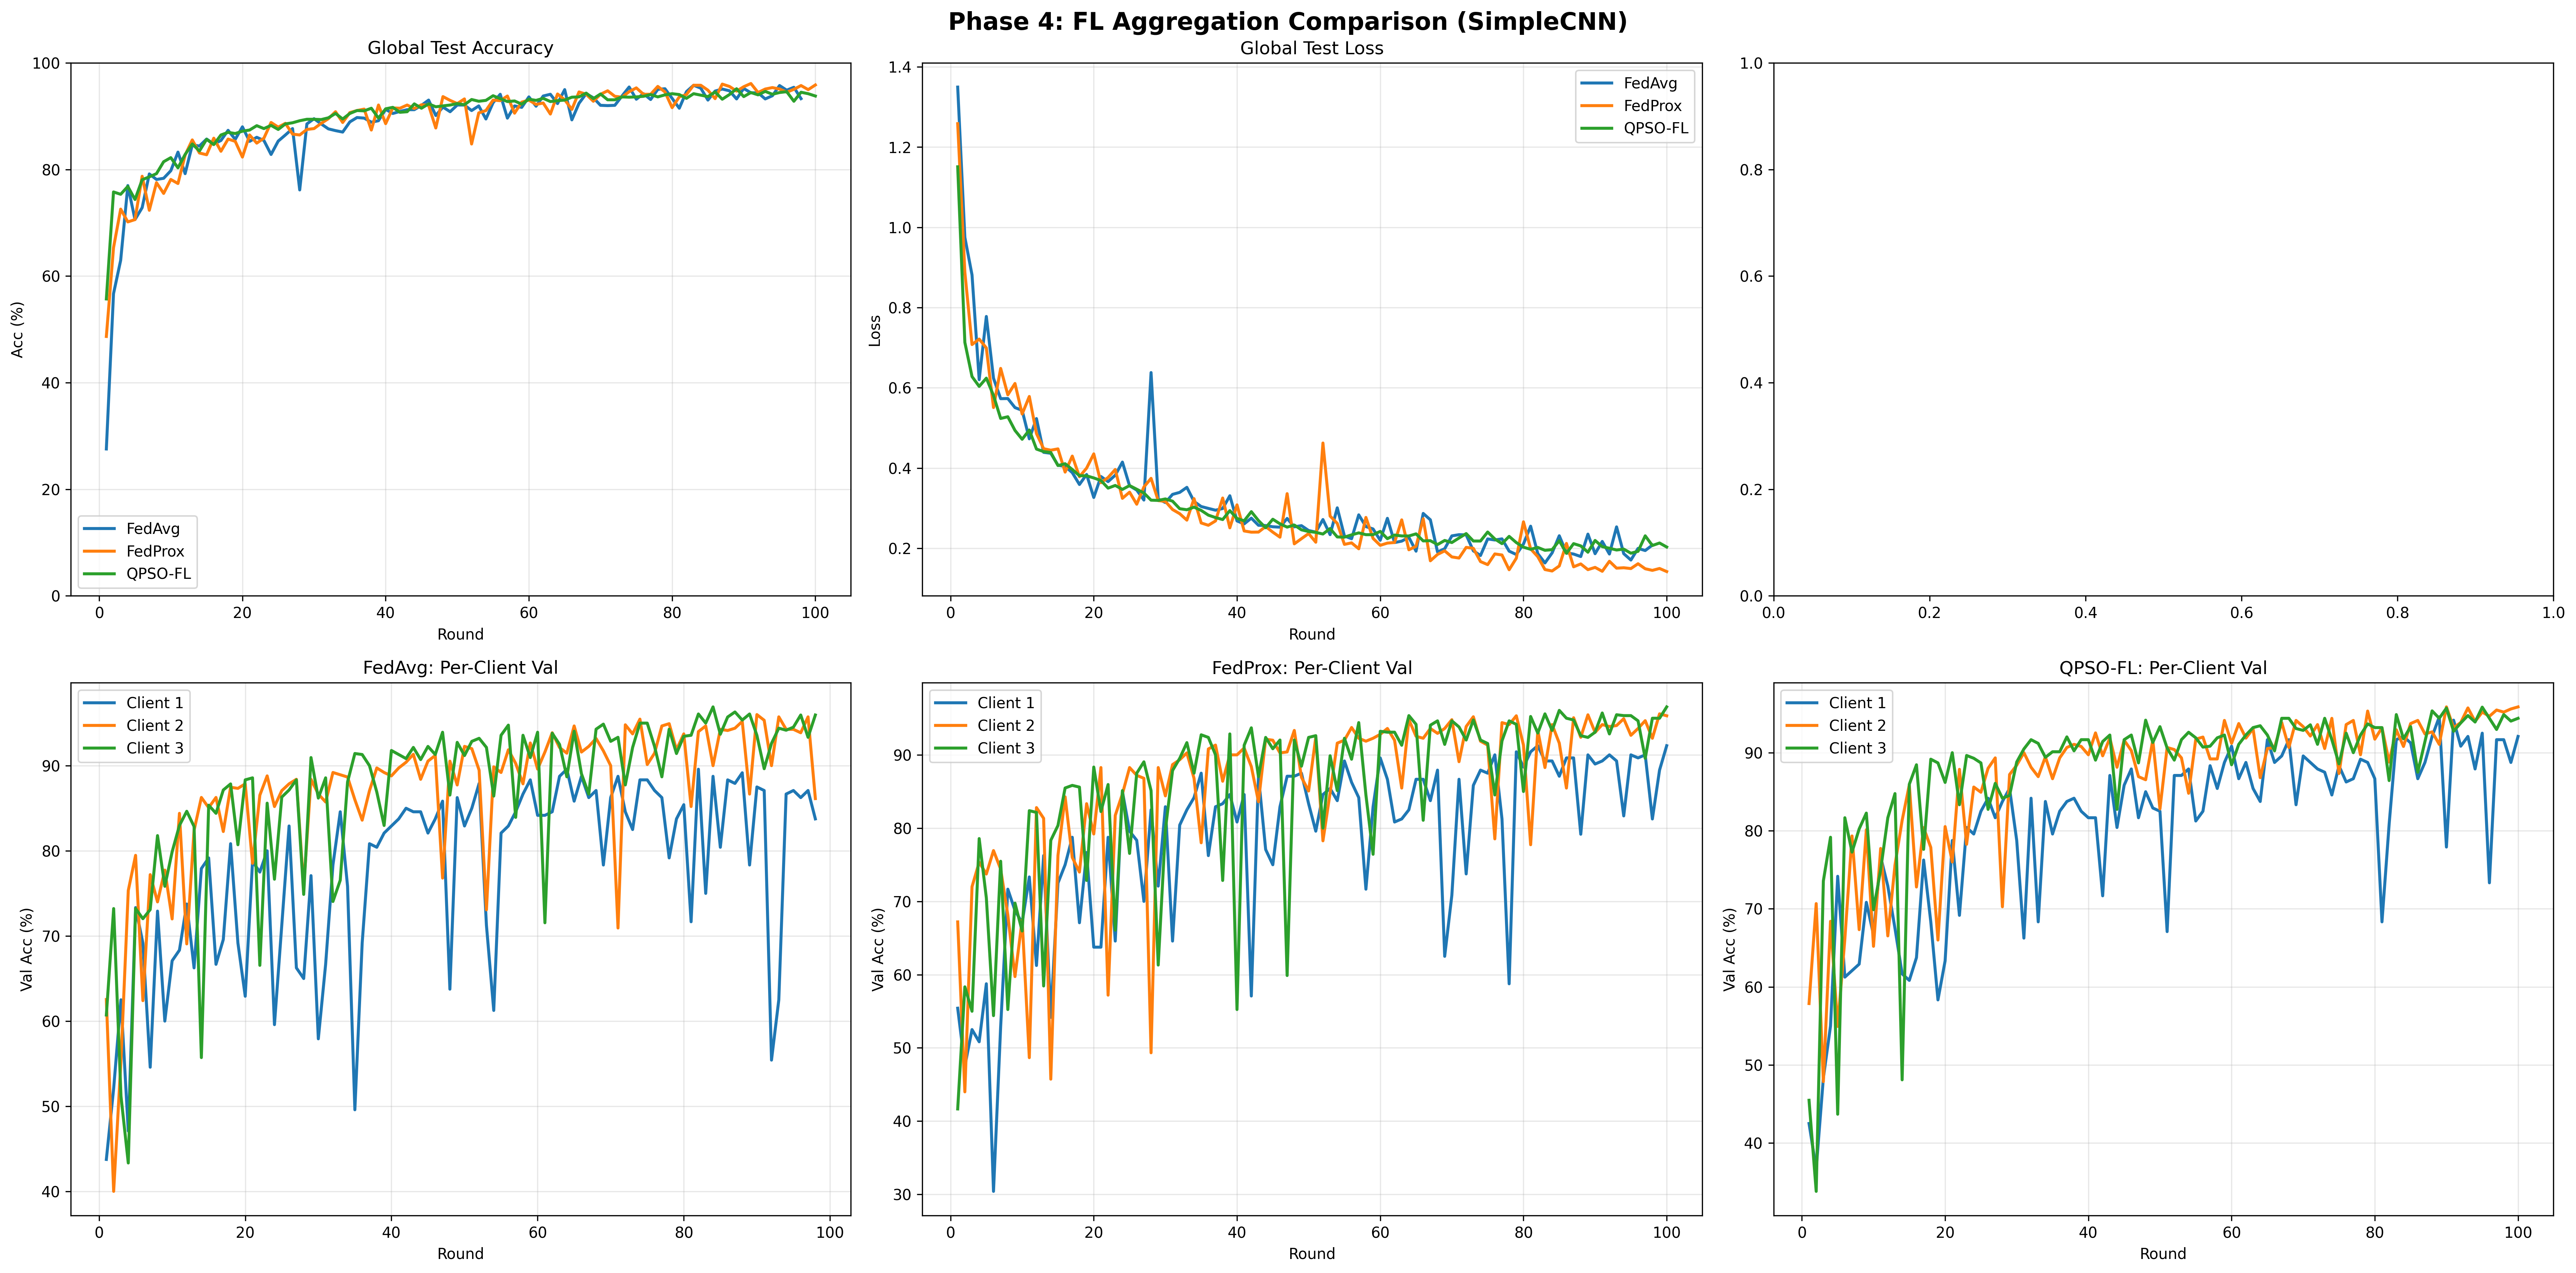
\includegraphics[width=\columnwidth]{s1_comparison.png}}
\caption{Accuracy and training loss curves over 100 rounds --- Setup~1
(Natural Heterogeneity). FedQPSO (green) exhibits markedly lower
round-to-round oscillation than FedAvg and FedProx, reflecting the
fitness-based rejection of unstable weight configurations.}
\label{fig:curves_s1}
\end{figure}

\begin{figure}[htbp]
\centerline{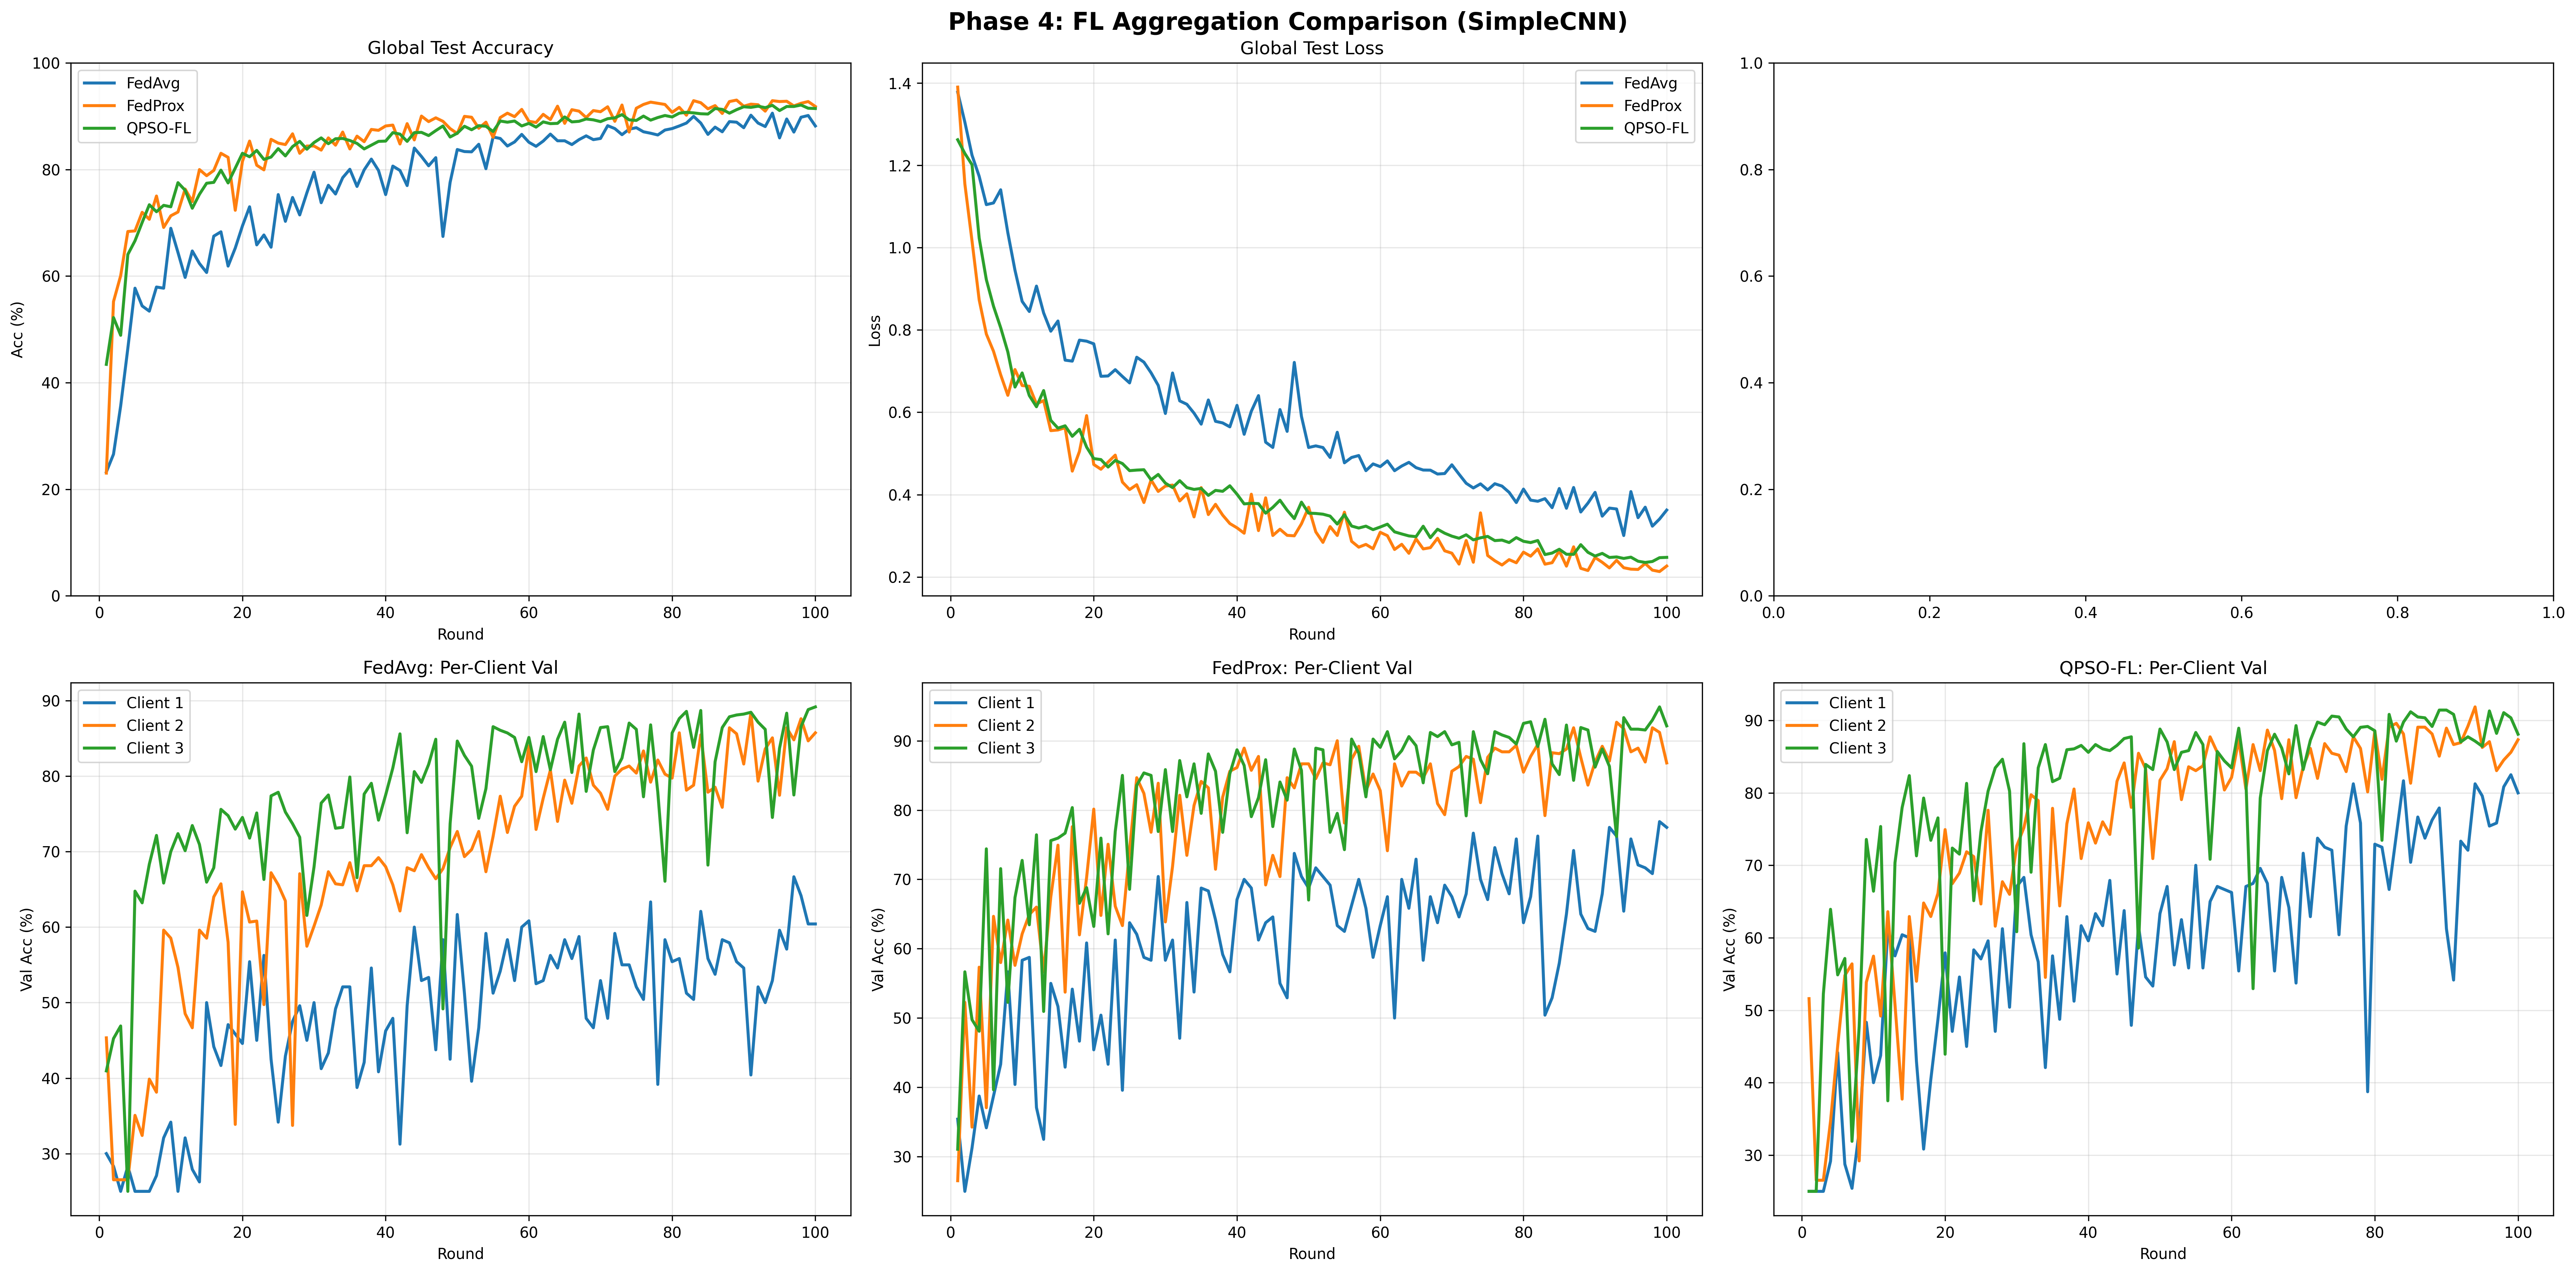
\includegraphics[width=\columnwidth]{s2_comparison.png}}
\caption{Accuracy and training loss curves over 100 rounds --- Setup~2
(Moderate Label Skew). FedAvg degrades substantially more under label skew,
while FedQPSO and FedProx maintain higher and more stable accuracy
trajectories throughout training.}
\label{fig:curves_s2}
\end{figure}

\subsection{Per-Class Classification Performance}

Table~\ref{tab:perclass} reports F1-score and Glioma recall for each
algorithm at its respective best-round model checkpoint.

\begin{table}[htbp]
\caption{Per-Class F1-Score and Glioma Recall at Best Checkpoint
(S1 = Setup~1, S2 = Setup~2)}
\label{tab:perclass}
\begin{center}
\renewcommand{\arraystretch}{1.15}
\begin{tabular}{llccc}
\hline
\textbf{Setup} & \textbf{Class} & \textbf{FedAvg} & \textbf{FedProx} &
\textbf{FedQPSO}\\
\hline
\multirow{5}{*}{S1 F1}
 & Glioma     & 0.9438 & 0.9420 & \textbf{0.9560}\\
 & Meningioma & 0.9378 & \textbf{0.9394} & 0.9211\\
 & No Tumor   & 0.9663 & \textbf{0.9790} & 0.9602\\
 & Pituitary  & 0.9828 & \textbf{0.9846} & 0.9686\\
 & Macro Avg  & 0.9577 & \textbf{0.9612} & 0.9515\\
\hline
\multirow{5}{*}{S2 F1}
 & Glioma     & 0.8841 & 0.9039 & \textbf{0.9089}\\
 & Meningioma & 0.8458 & \textbf{0.8921} & 0.8727\\
 & No Tumor   & 0.9447 & \textbf{0.9554} & 0.9528\\
 & Pituitary  & 0.9491 & \textbf{0.9689} & 0.9507\\
 & Macro Avg  & 0.9059 & \textbf{0.9301} & 0.9213\\
\hline
\multirow{2}{*}{Recall}
 & Glioma (S1) & 0.9118 & 0.9186 & \textbf{0.9593}\\
 & Glioma (S2) & 0.8371 & 0.8620 & \textbf{0.8914}\\
\hline
\end{tabular}
\end{center}
\end{table}

FedQPSO achieves the \textbf{highest Glioma F1 and recall in both setups}
--- the most clinically critical class, where missed diagnoses carry
potentially fatal consequences. Under label skew, FedQPSO's Glioma recall
improvement over FedAvg (5.43\,pp) corresponds to approximately 24
additional correctly identified glioma cases per 1,000 patients.
FedProx leads on Meningioma, No Tumor, and Pituitary in both conditions,
indicating that when class distributions are homogeneous, the proximal
regularizer provides an accuracy benefit FedQPSO does not match.

\subsection{Client Fairness}
\label{sec:fairness}

Table~\ref{tab:fairness} presents client fairness metrics; Figs.~\ref{fig:fairness_s1}
and~\ref{fig:fairness_s2} visualize per-client accuracy distributions over
all training rounds.

\begin{table}[htbp]
\caption{Client Fairness Metrics (Final Round and At-Peak-Round)}
\label{tab:fairness}
\begin{center}
\renewcommand{\arraystretch}{1.15}
\begin{tabular}{llccc}
\hline
\textbf{Setup} & \textbf{Metric} & \textbf{FedAvg} & \textbf{FedProx} &
\textbf{FedQPSO}\\
\hline
\multirow{4}{*}{S1}
 & Cl.\ 1 final (\%)       & 83.75 & 91.25 & \textbf{92.08}\\
 & Client $\sigma$ final   & 5.28\% & 2.27\% & \textbf{1.56\%}\\
 & Max$-$Min gap (pp)      & 12.20 & 5.30 & \textbf{2.32}\\
 & Client $\sigma$ at peak & 9.50\% & 2.79\% & \textbf{1.62\%}\\
\hline
\multirow{4}{*}{S2}
 & Cl.\ 1 final (\%)       & 60.42 & 77.50 & \textbf{80.00}\\
 & Client $\sigma$ final   & 12.82\% & 6.05\% & \textbf{3.65\%}\\
 & Max$-$Min gap (pp)      & 28.75 & 14.64 & \textbf{8.10}\\
 & Client $\sigma$ at peak & 13.38\% & 12.07\% & \textbf{4.23\%}\\
\hline
\end{tabular}
\end{center}
\end{table}

\begin{figure}[htbp]
\centerline{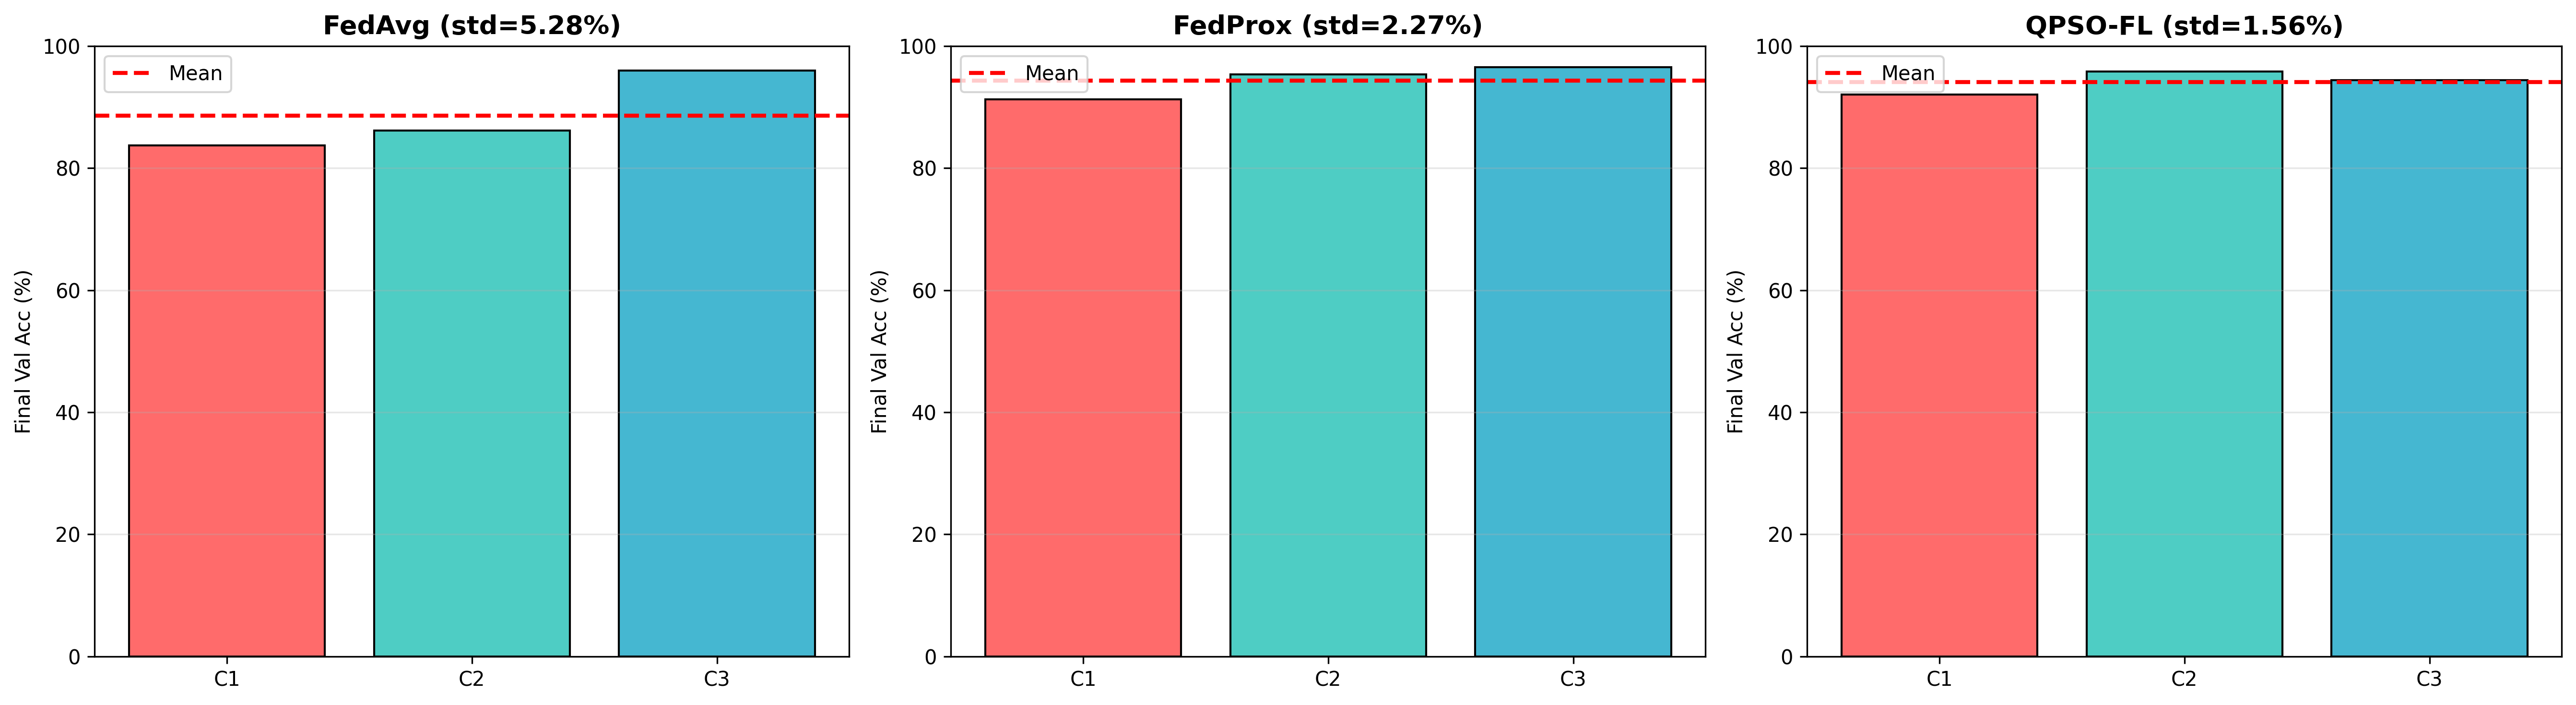
\includegraphics[width=\columnwidth]{s1_fairness.png}}
\caption{Per-client validation accuracy over all rounds --- Setup~1
(Natural Heterogeneity). When FedAvg peaks globally at 95.80\% (round~83),
Client~1 is simultaneously at 75.00\% --- a 20.80\,pp hidden inequity.
FedQPSO keeps all clients within 2.32\,pp at convergence.}
\label{fig:fairness_s1}
\end{figure}

\begin{figure}[htbp]
\centerline{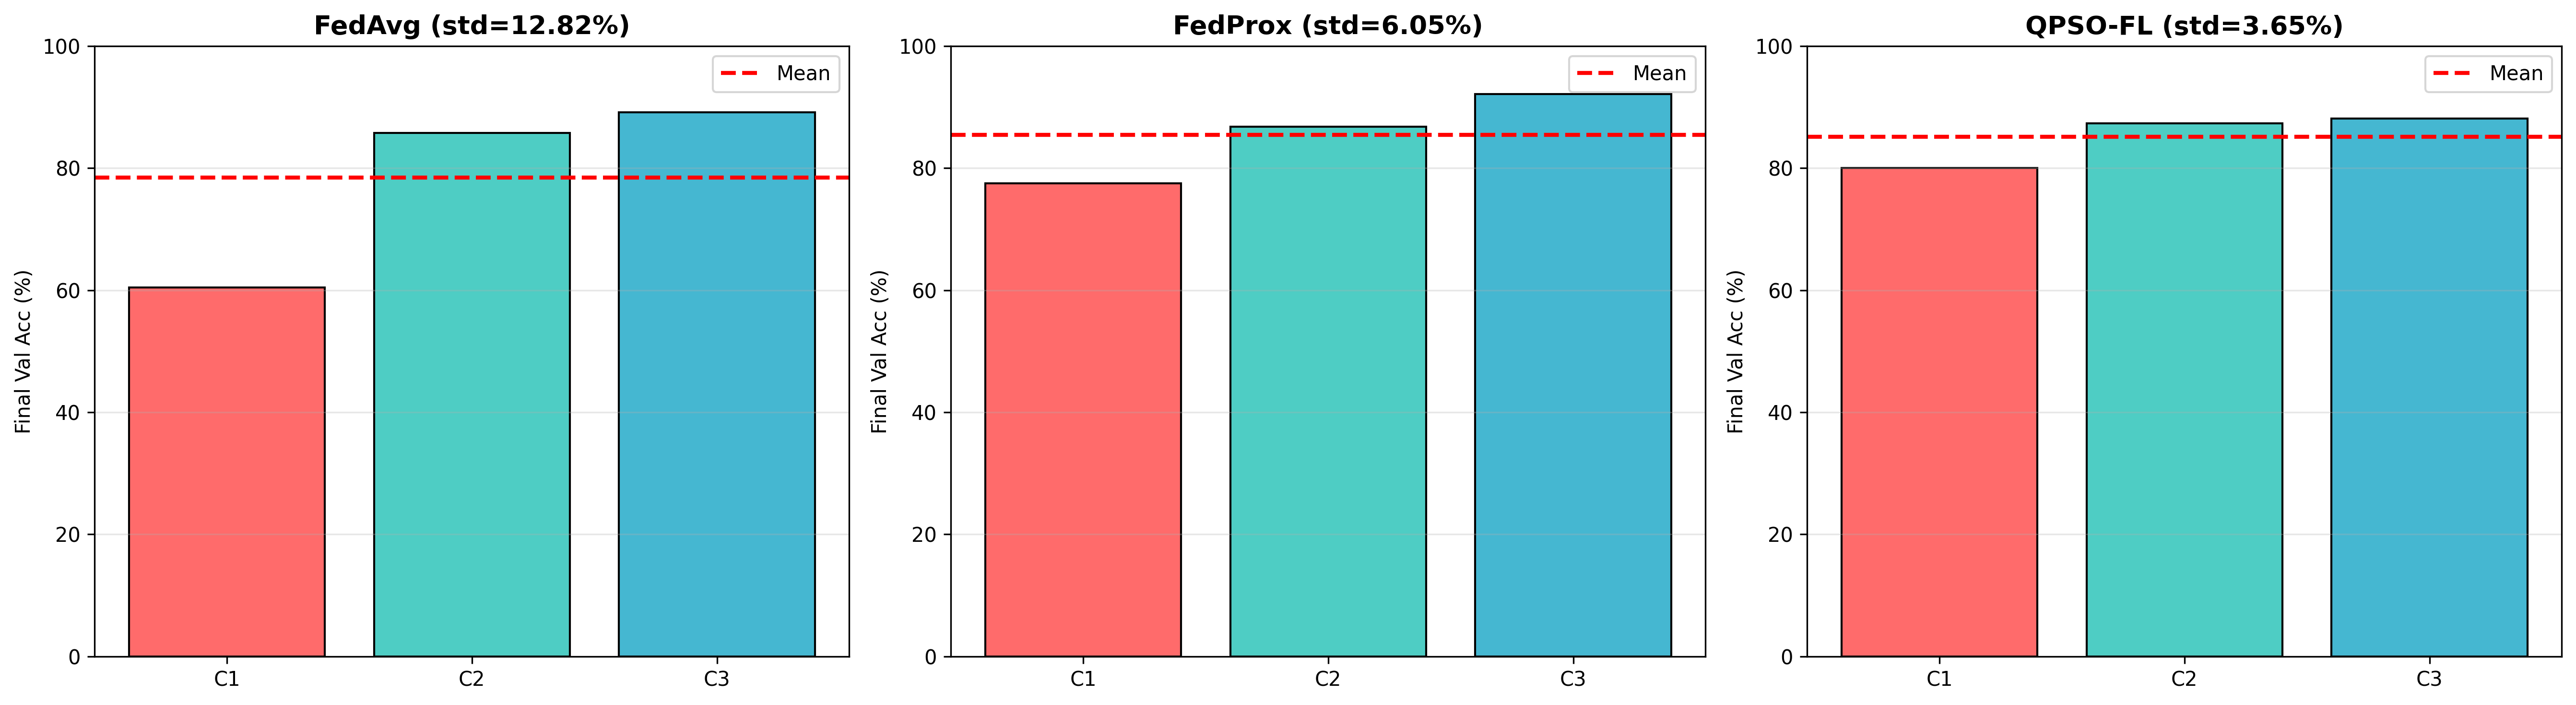
\includegraphics[width=\columnwidth]{s2_fairness.png}}
\caption{Per-client validation accuracy over all rounds --- Setup~2
(Label Skew). Under FedAvg, Client~1 converges to just 60.42\% --- barely
above chance for a 4-class problem. FedQPSO is the only method keeping
Client~1 at or above 80\% at convergence.}
\label{fig:fairness_s2}
\end{figure}

The most clinically significant result: at FedAvg's peak global accuracy of
90.56\% (Setup~2, round~94), Client~1's concurrent validation accuracy was
\textbf{52.92\%} --- barely above random for a 4-class problem. At FedQPSO's
peak (92.09\%, round~98), Client~1 was at \textbf{80.83\%} --- a 27.91\,pp
improvement for the weakest hospital at the same moment of best global
performance.

FedQPSO reduces FedAvg's max-min gap by \textbf{81\%} in Setup~1
(12.20 $\to$ 2.32\,pp) and \textbf{72\%} in Setup~2 (28.75 $\to$
8.10\,pp), and exceeds FedProx's fairness improvement by 45--56\% on the
same metric. The QPSO--FedProx fairness gap \emph{widens} from 0.71\,pp to
2.40\,pp in client $\sigma$ as heterogeneity increases --- the mechanism
becomes more effective under harder conditions.

\subsection{Statistical Significance}

Table~\ref{tab:stats} summarizes paired two-tailed $t$-tests on per-round
global accuracy sequences.

\begin{table}[htbp]
\caption{Statistical Significance: Paired $t$-Test on Per-Round Accuracy}
\label{tab:stats}
\begin{center}
\begin{tabular}{llcccl}
\hline
\textbf{Setup} & \textbf{Comparison} & $t$ & $p$ & $d$ & \textbf{Sig.}\\
\hline
S1 & FedAvg vs FedQPSO  & 3.43  & 0.000882 & 0.35 & \checkmark \\
S1 & FedAvg vs FedProx  & 1.72  & 0.0879   & 0.17 & $\times$   \\
S2 & FedAvg vs FedQPSO  & 12.59 & $2.91\!\times\!10^{-22}$ & 1.26 & \checkmark \\
S2 & FedAvg vs FedProx  & 13.39 & $5.86\!\times\!10^{-24}$ & 1.34 & \checkmark \\
\hline
\multicolumn{6}{l}{\small \checkmark: $p < 0.05$; \quad $d$: Cohen's $d$ effect size.}
\end{tabular}
\end{center}
\end{table}

Under natural heterogeneity, \textbf{FedQPSO is the only method that
statistically significantly outperforms FedAvg} ($p = 0.000882$, $d = 0.35$).
FedProx fails to reach significance ($p = 0.088$, $d = 0.17$) --- its
proximal term is insufficient when distributions are only mildly
heterogeneous. Under label skew, both FedQPSO and FedProx achieve
overwhelming statistical separation from FedAvg (Cohen's $d > 1.2$ for
both). The jump in effect size from $d = 0.35$ (Setup~1) to $d = 1.26$
(Setup~2) confirms that FedQPSO's advantage scales with heterogeneity
severity.

\subsection{ROC-AUC Analysis}

Table~\ref{tab:auc} reports ROC-AUC for each class and the micro-average.
Corresponding ROC curves are shown in Figs.~\ref{fig:roc_s1}
and~\ref{fig:roc_s2}.

\begin{table}[htbp]
\caption{ROC-AUC Per Class and Micro-Average}
\label{tab:auc}
\begin{center}
\begin{tabular}{lcccccc}
\hline
& \multicolumn{3}{c}{\textbf{Setup 1}} &
  \multicolumn{3}{c}{\textbf{Setup 2}}\\
\cmidrule(lr){2-4}\cmidrule(lr){5-7}
\textbf{Class} & FA & FP & \textbf{FQ} & FA & FP & \textbf{FQ}\\
\hline
Glioma     & 0.988 & 0.988 & \textbf{0.991} & 0.977 & 0.983 & \textbf{0.985}\\
Meningioma & 0.992 & \textbf{0.993} & 0.986 & 0.970 & \textbf{0.981} & 0.978\\
No Tumor   & 0.998 & \textbf{0.999} & 0.995 & 0.996 & \textbf{0.997} & \textbf{0.997}\\
Pituitary  & \textbf{0.999} & \textbf{0.999} & 0.998 & 0.996 & \textbf{0.997} & \textbf{0.997}\\
Micro Avg  & 0.995 & \textbf{0.996} & 0.993 & 0.986 & \textbf{0.991} & 0.990\\
\hline
\multicolumn{7}{l}{\small FA=FedAvg, FP=FedProx, FQ=FedQPSO.}
\end{tabular}
\end{center}
\end{table}

All methods achieve clinically excellent AUC across all classes in both
setups --- no value falls below 0.970. FedQPSO leads Glioma AUC in
\emph{both} conditions (0.991; 0.985), consistent with its superior Glioma
recall. Differences in overall micro-average AUC are small ($\leq$0.003),
indicating that the primary differentiator between methods is fairness, not
discrimination ability.

\begin{figure}[htbp]
\centerline{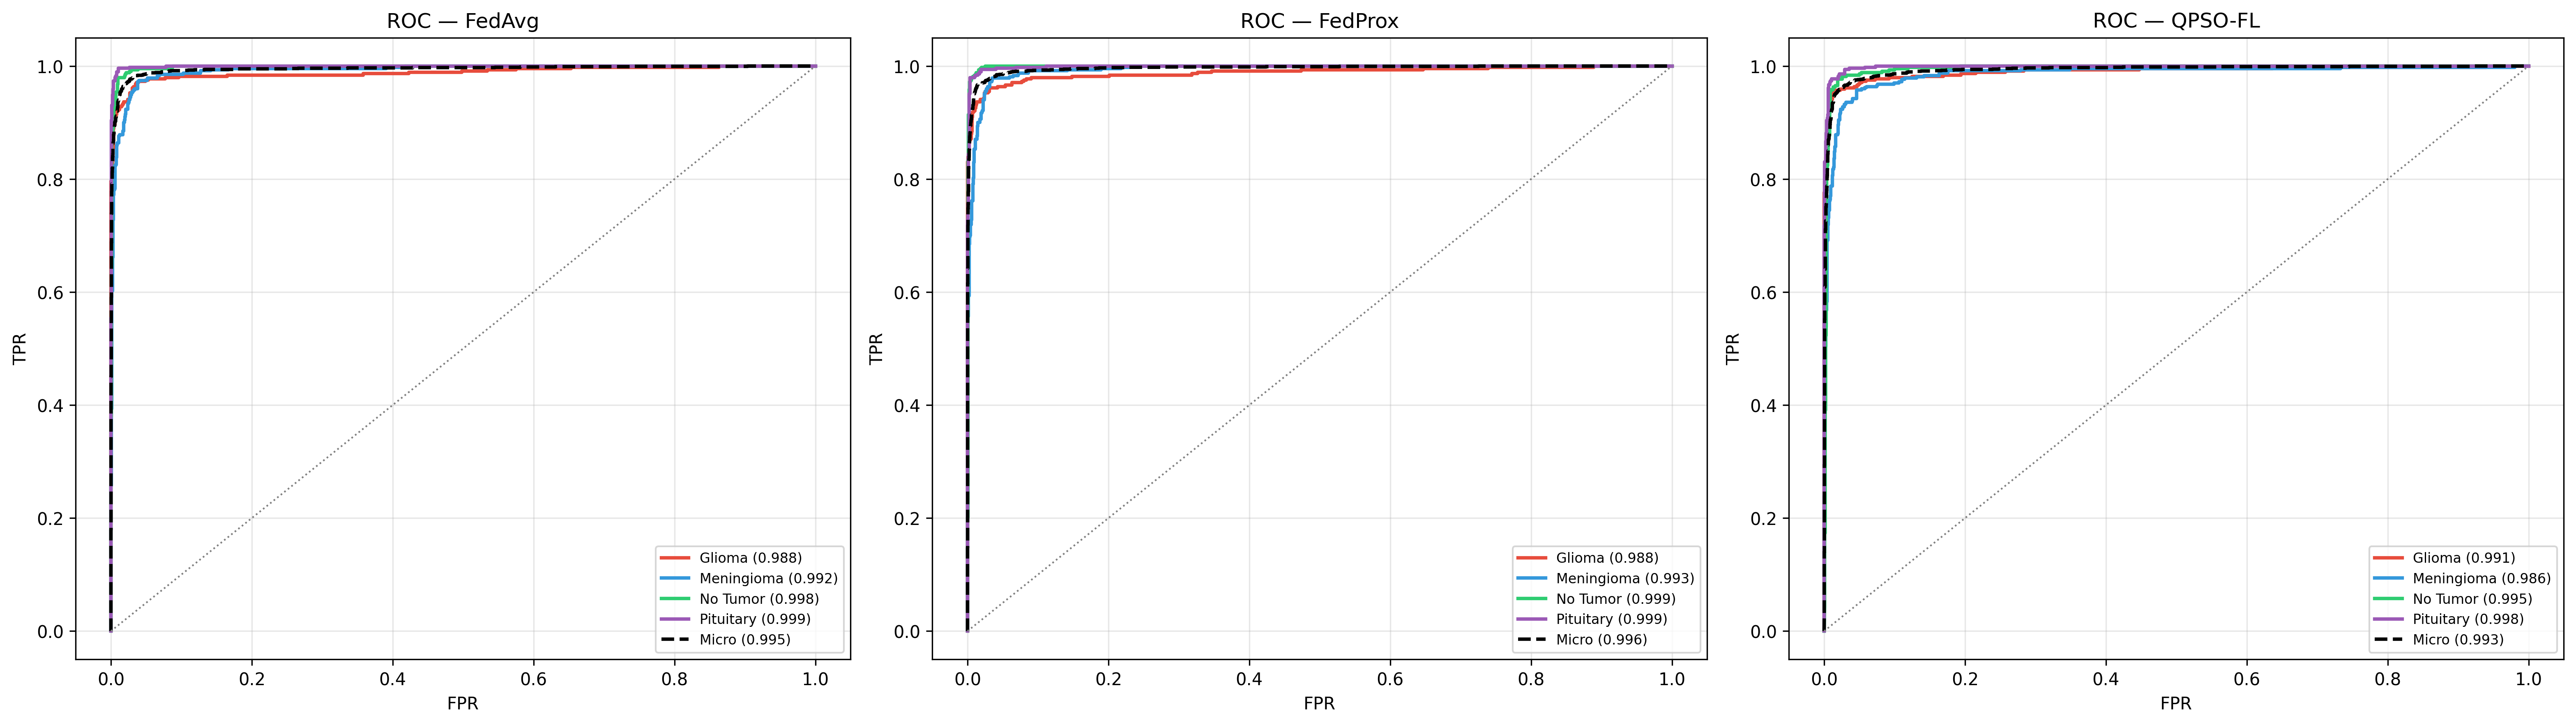
\includegraphics[width=\columnwidth]{s1_roc_auc.png}}
\caption{ROC-AUC curves --- Setup~1. All methods achieve AUC $>$ 0.986 for
every class. FedQPSO leads the Glioma curve (AUC = 0.991), the most
clinically critical class.}
\label{fig:roc_s1}
\end{figure}

\begin{figure}[htbp]
\centerline{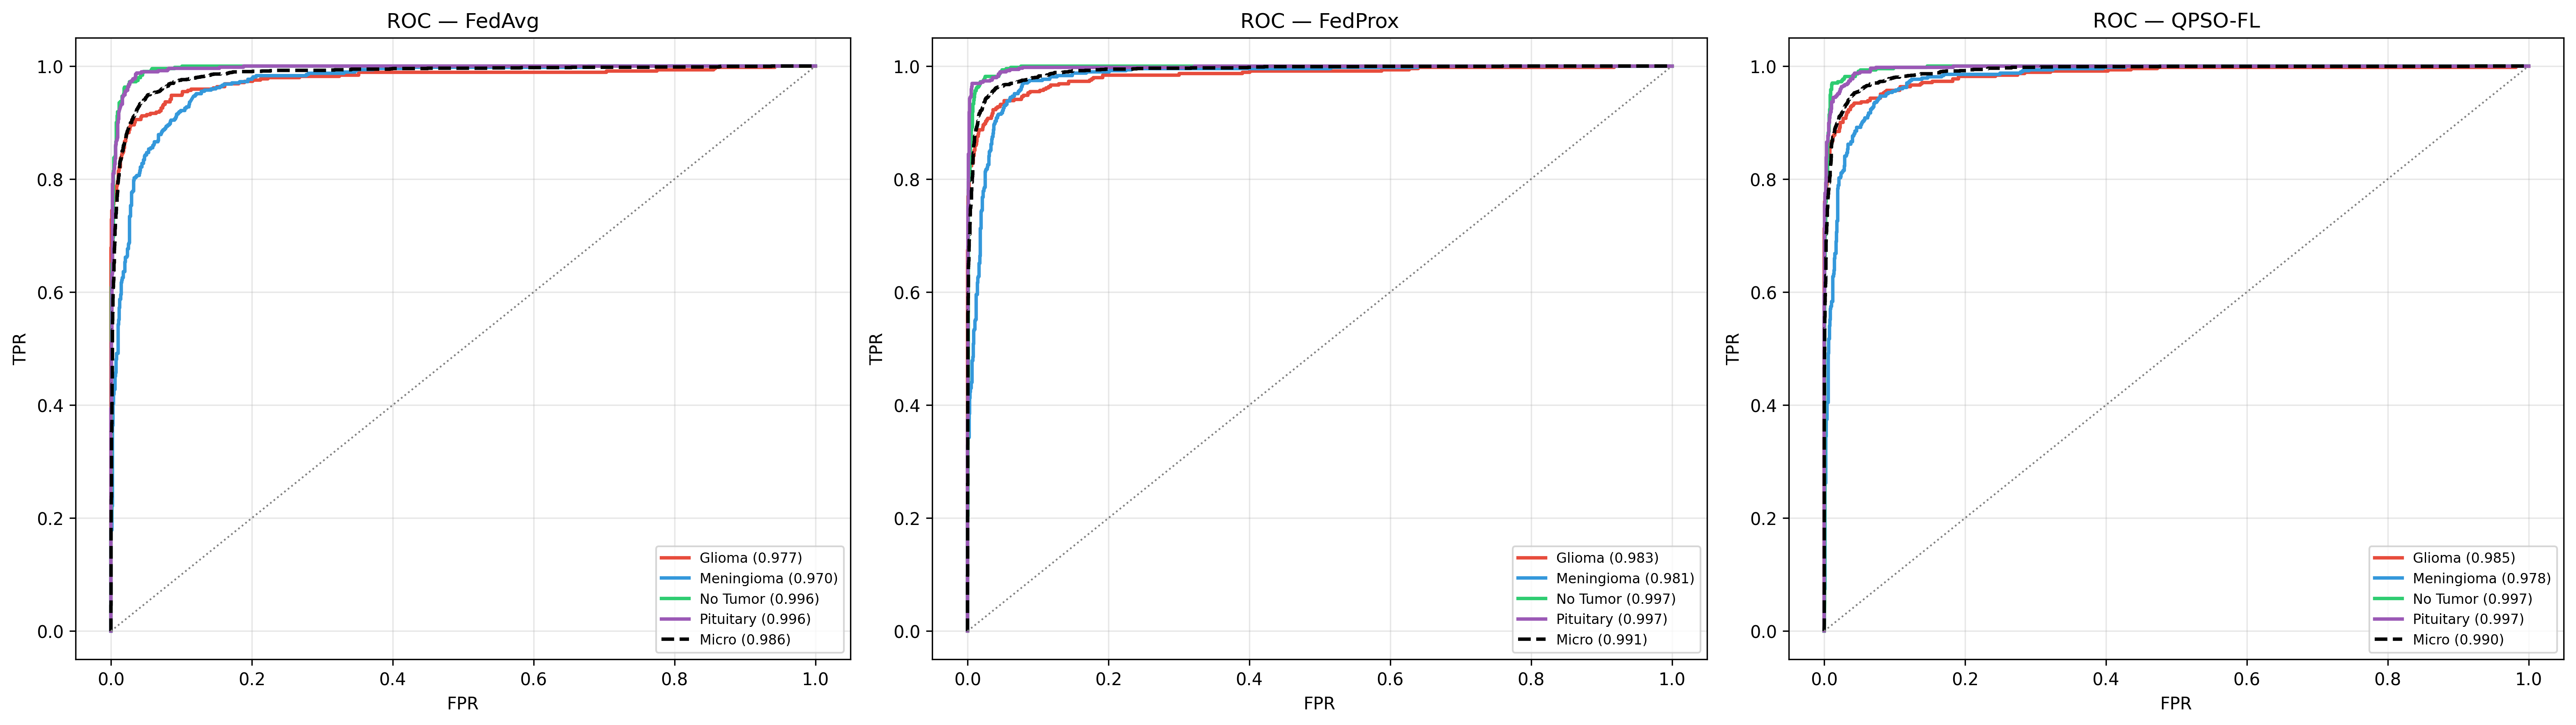
\includegraphics[width=\columnwidth]{s2_roc_auc.png}}
\caption{ROC-AUC curves --- Setup~2. Under label skew FedAvg's Meningioma
AUC drops to 0.970; FedQPSO and FedProx maintain above 0.978 for all
classes.}
\label{fig:roc_s2}
\end{figure}

\subsection{Confusion Matrices}

Figs.~\ref{fig:cm_s1} and~\ref{fig:cm_s2} show confusion matrices at
each method's best-round checkpoint.

\begin{figure}[htbp]
\centerline{%
  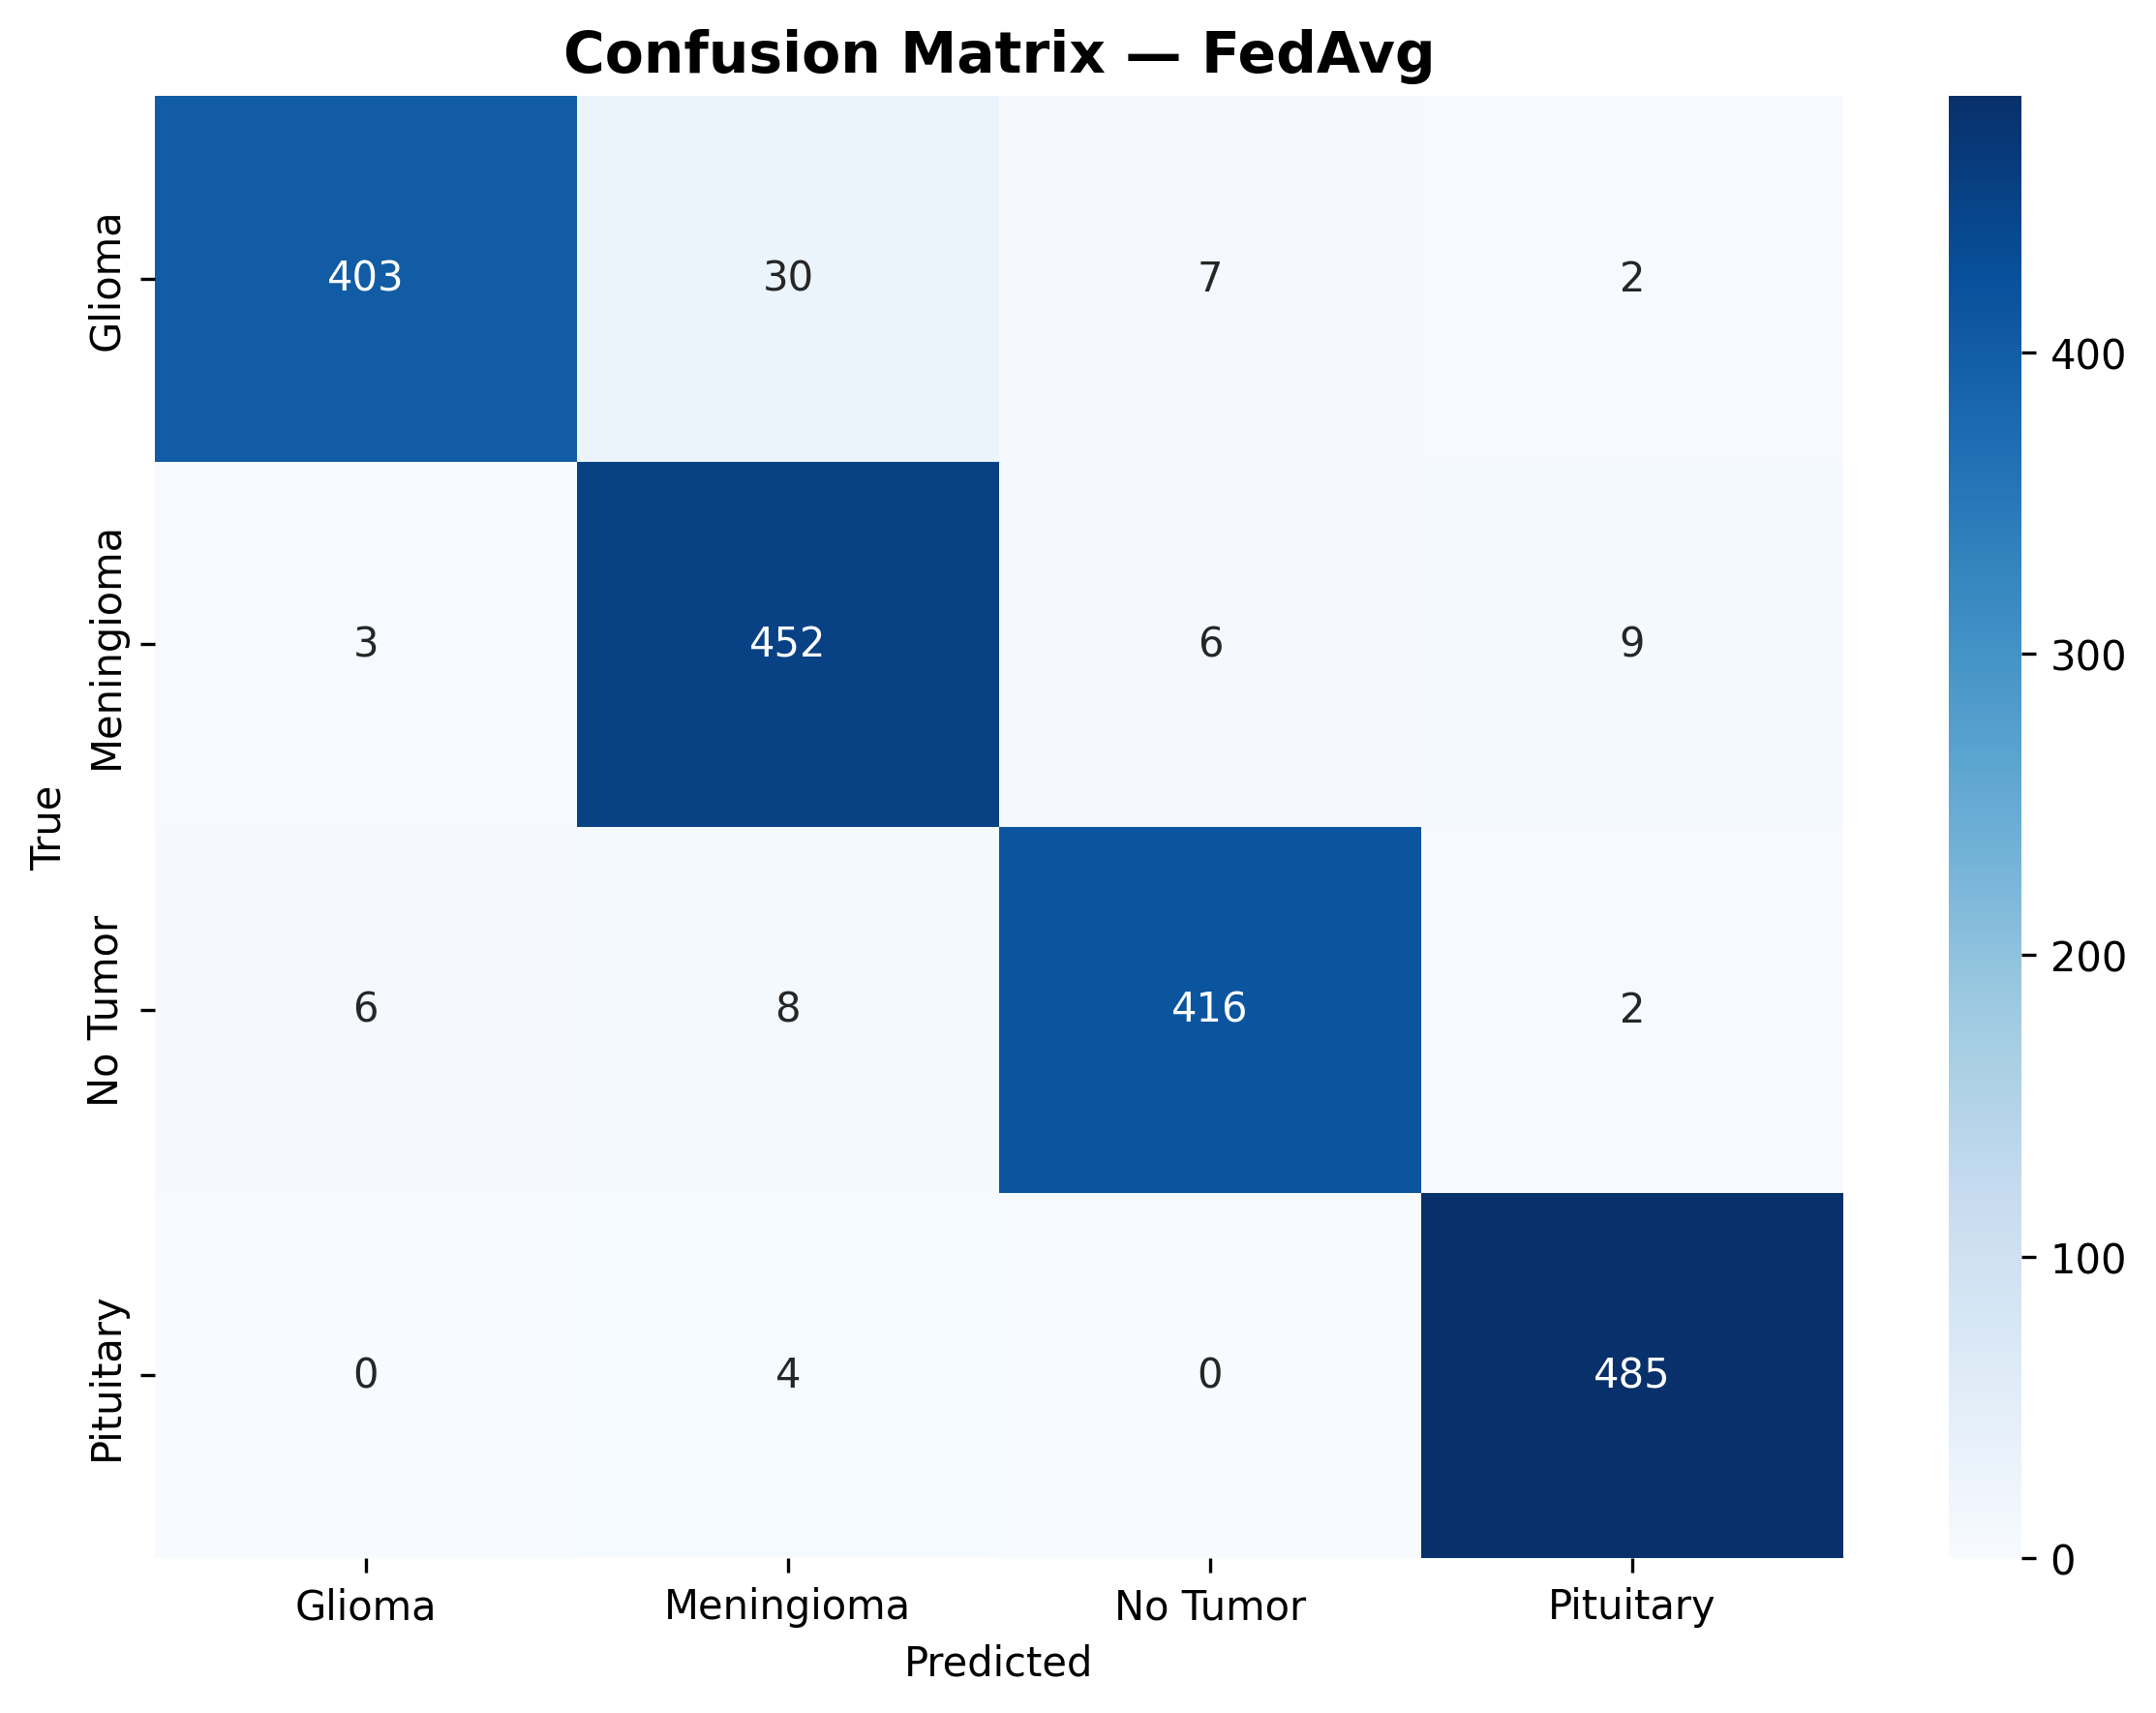
\includegraphics[width=0.32\columnwidth]{s1_cm_fedavg.png}%
  \hfill
  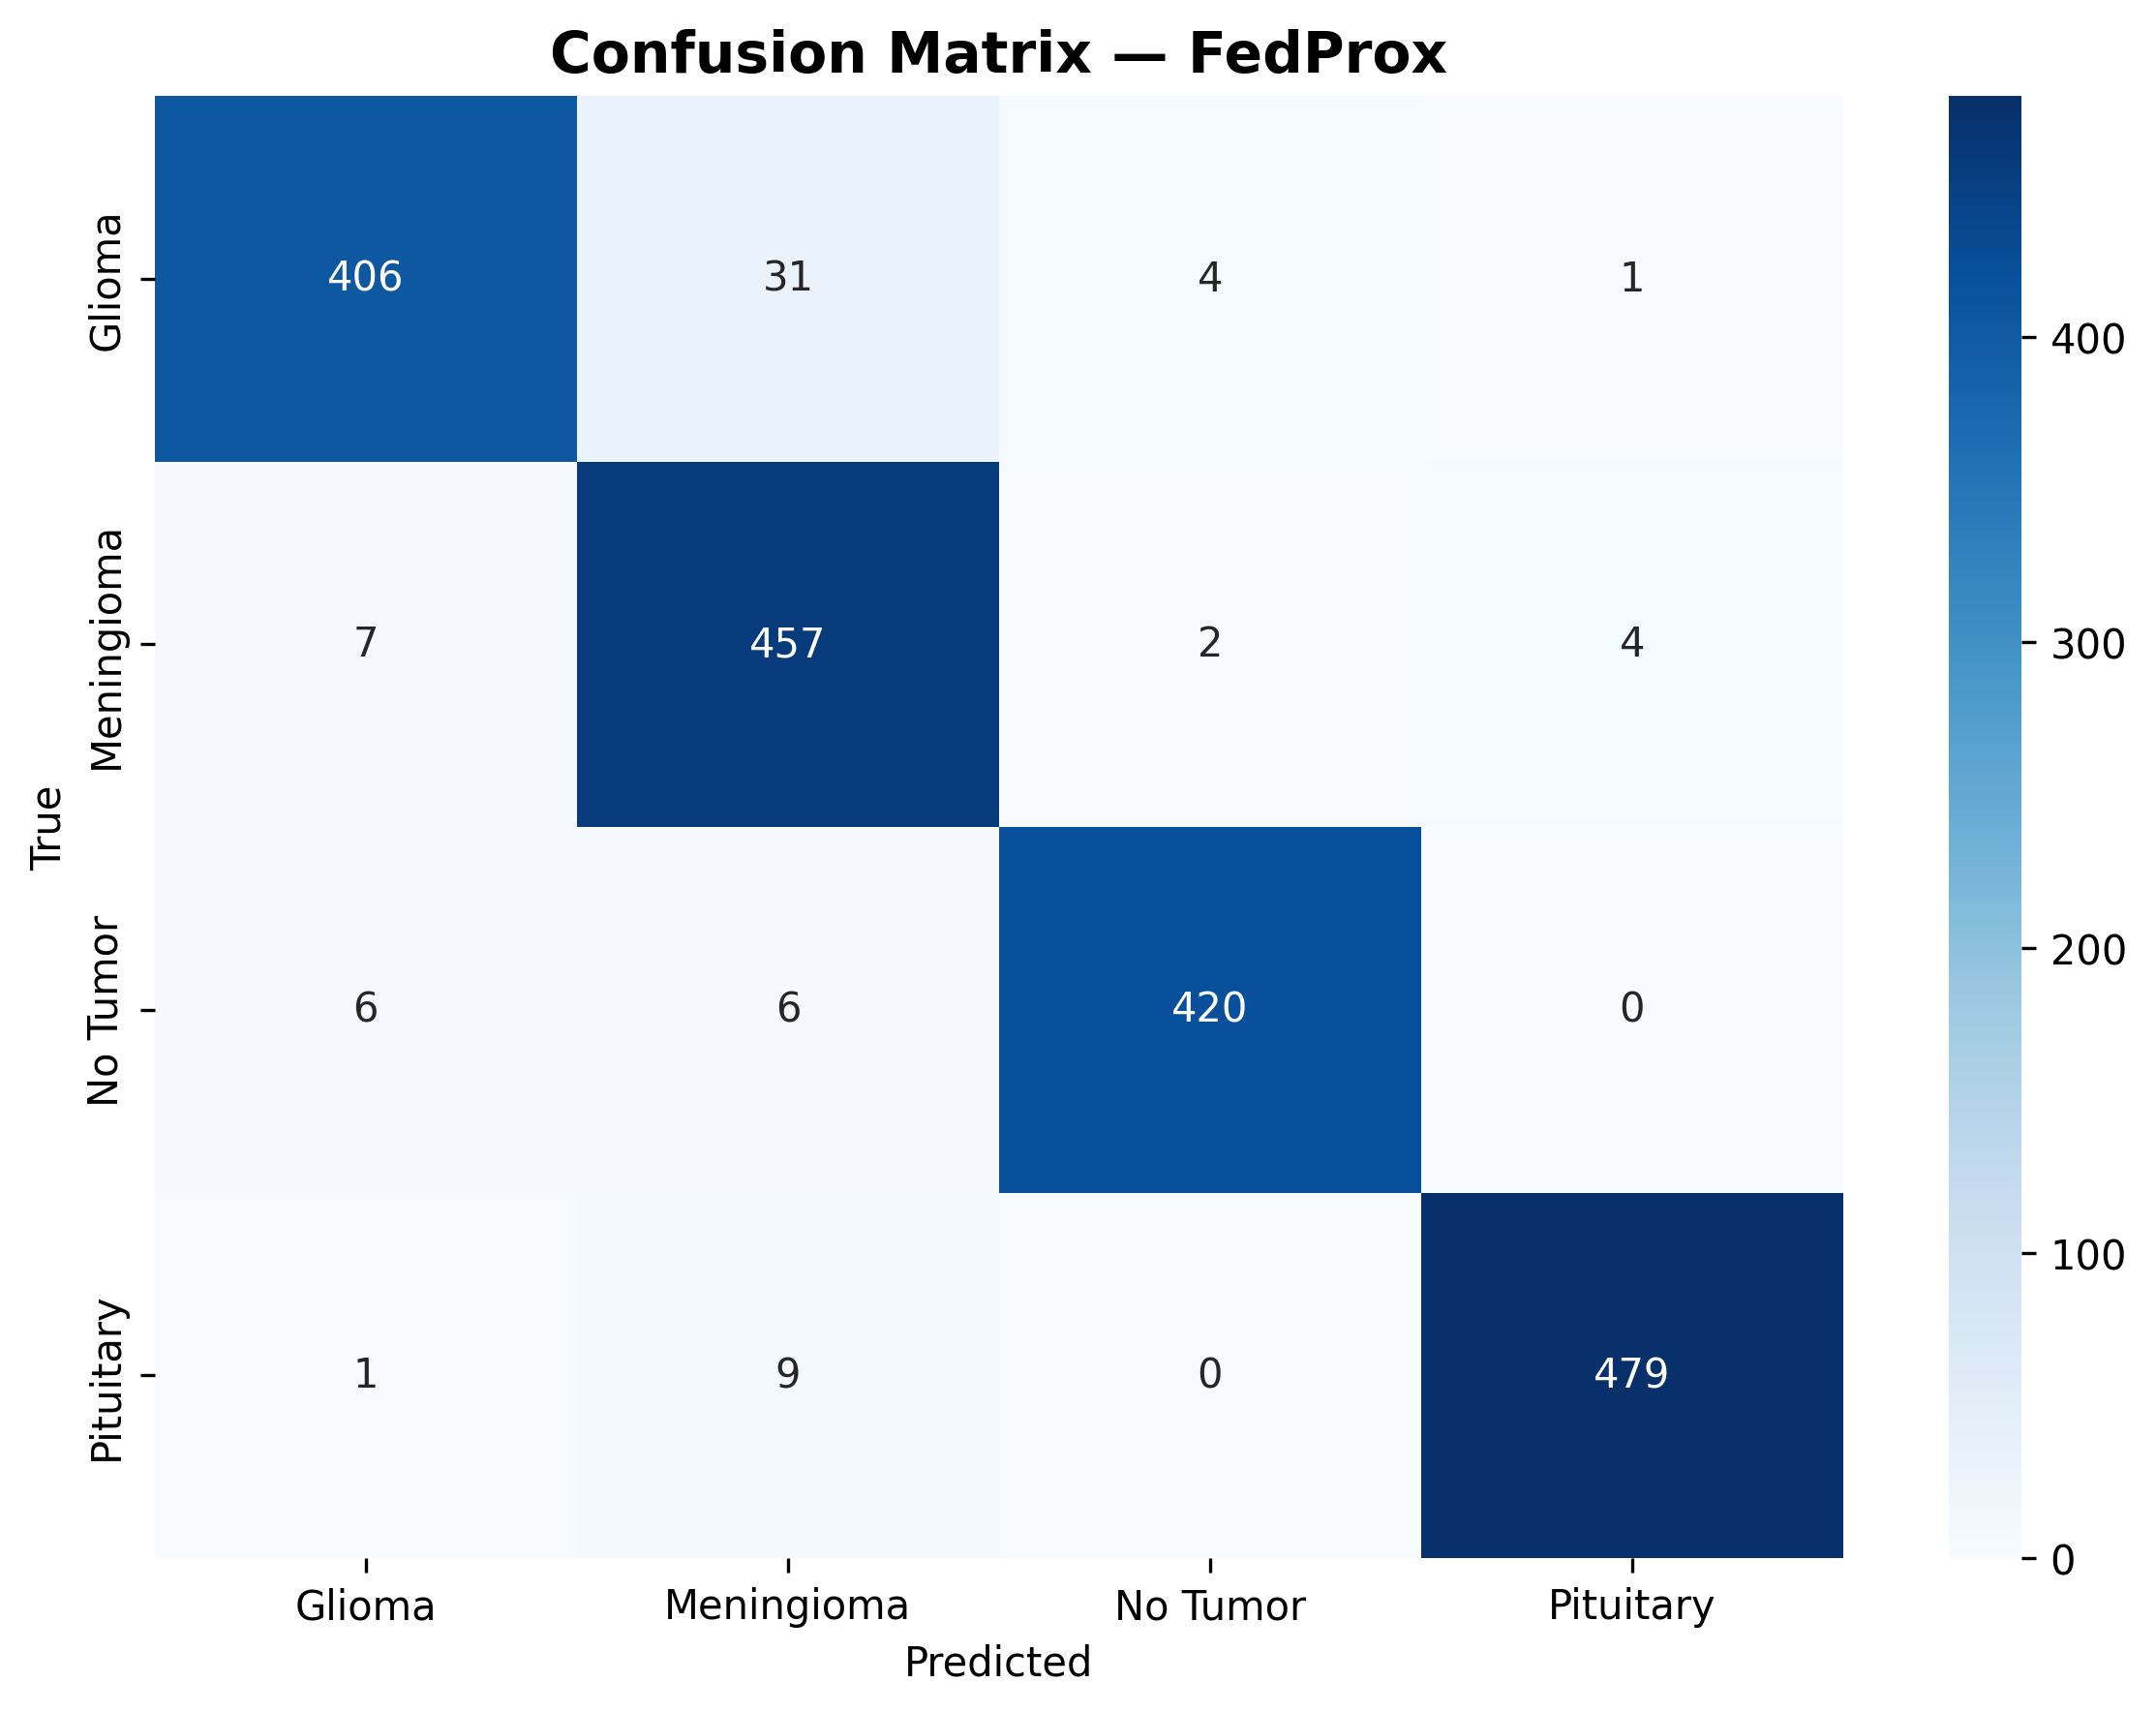
\includegraphics[width=0.32\columnwidth]{s1_cm_fedprox.png}%
  \hfill
  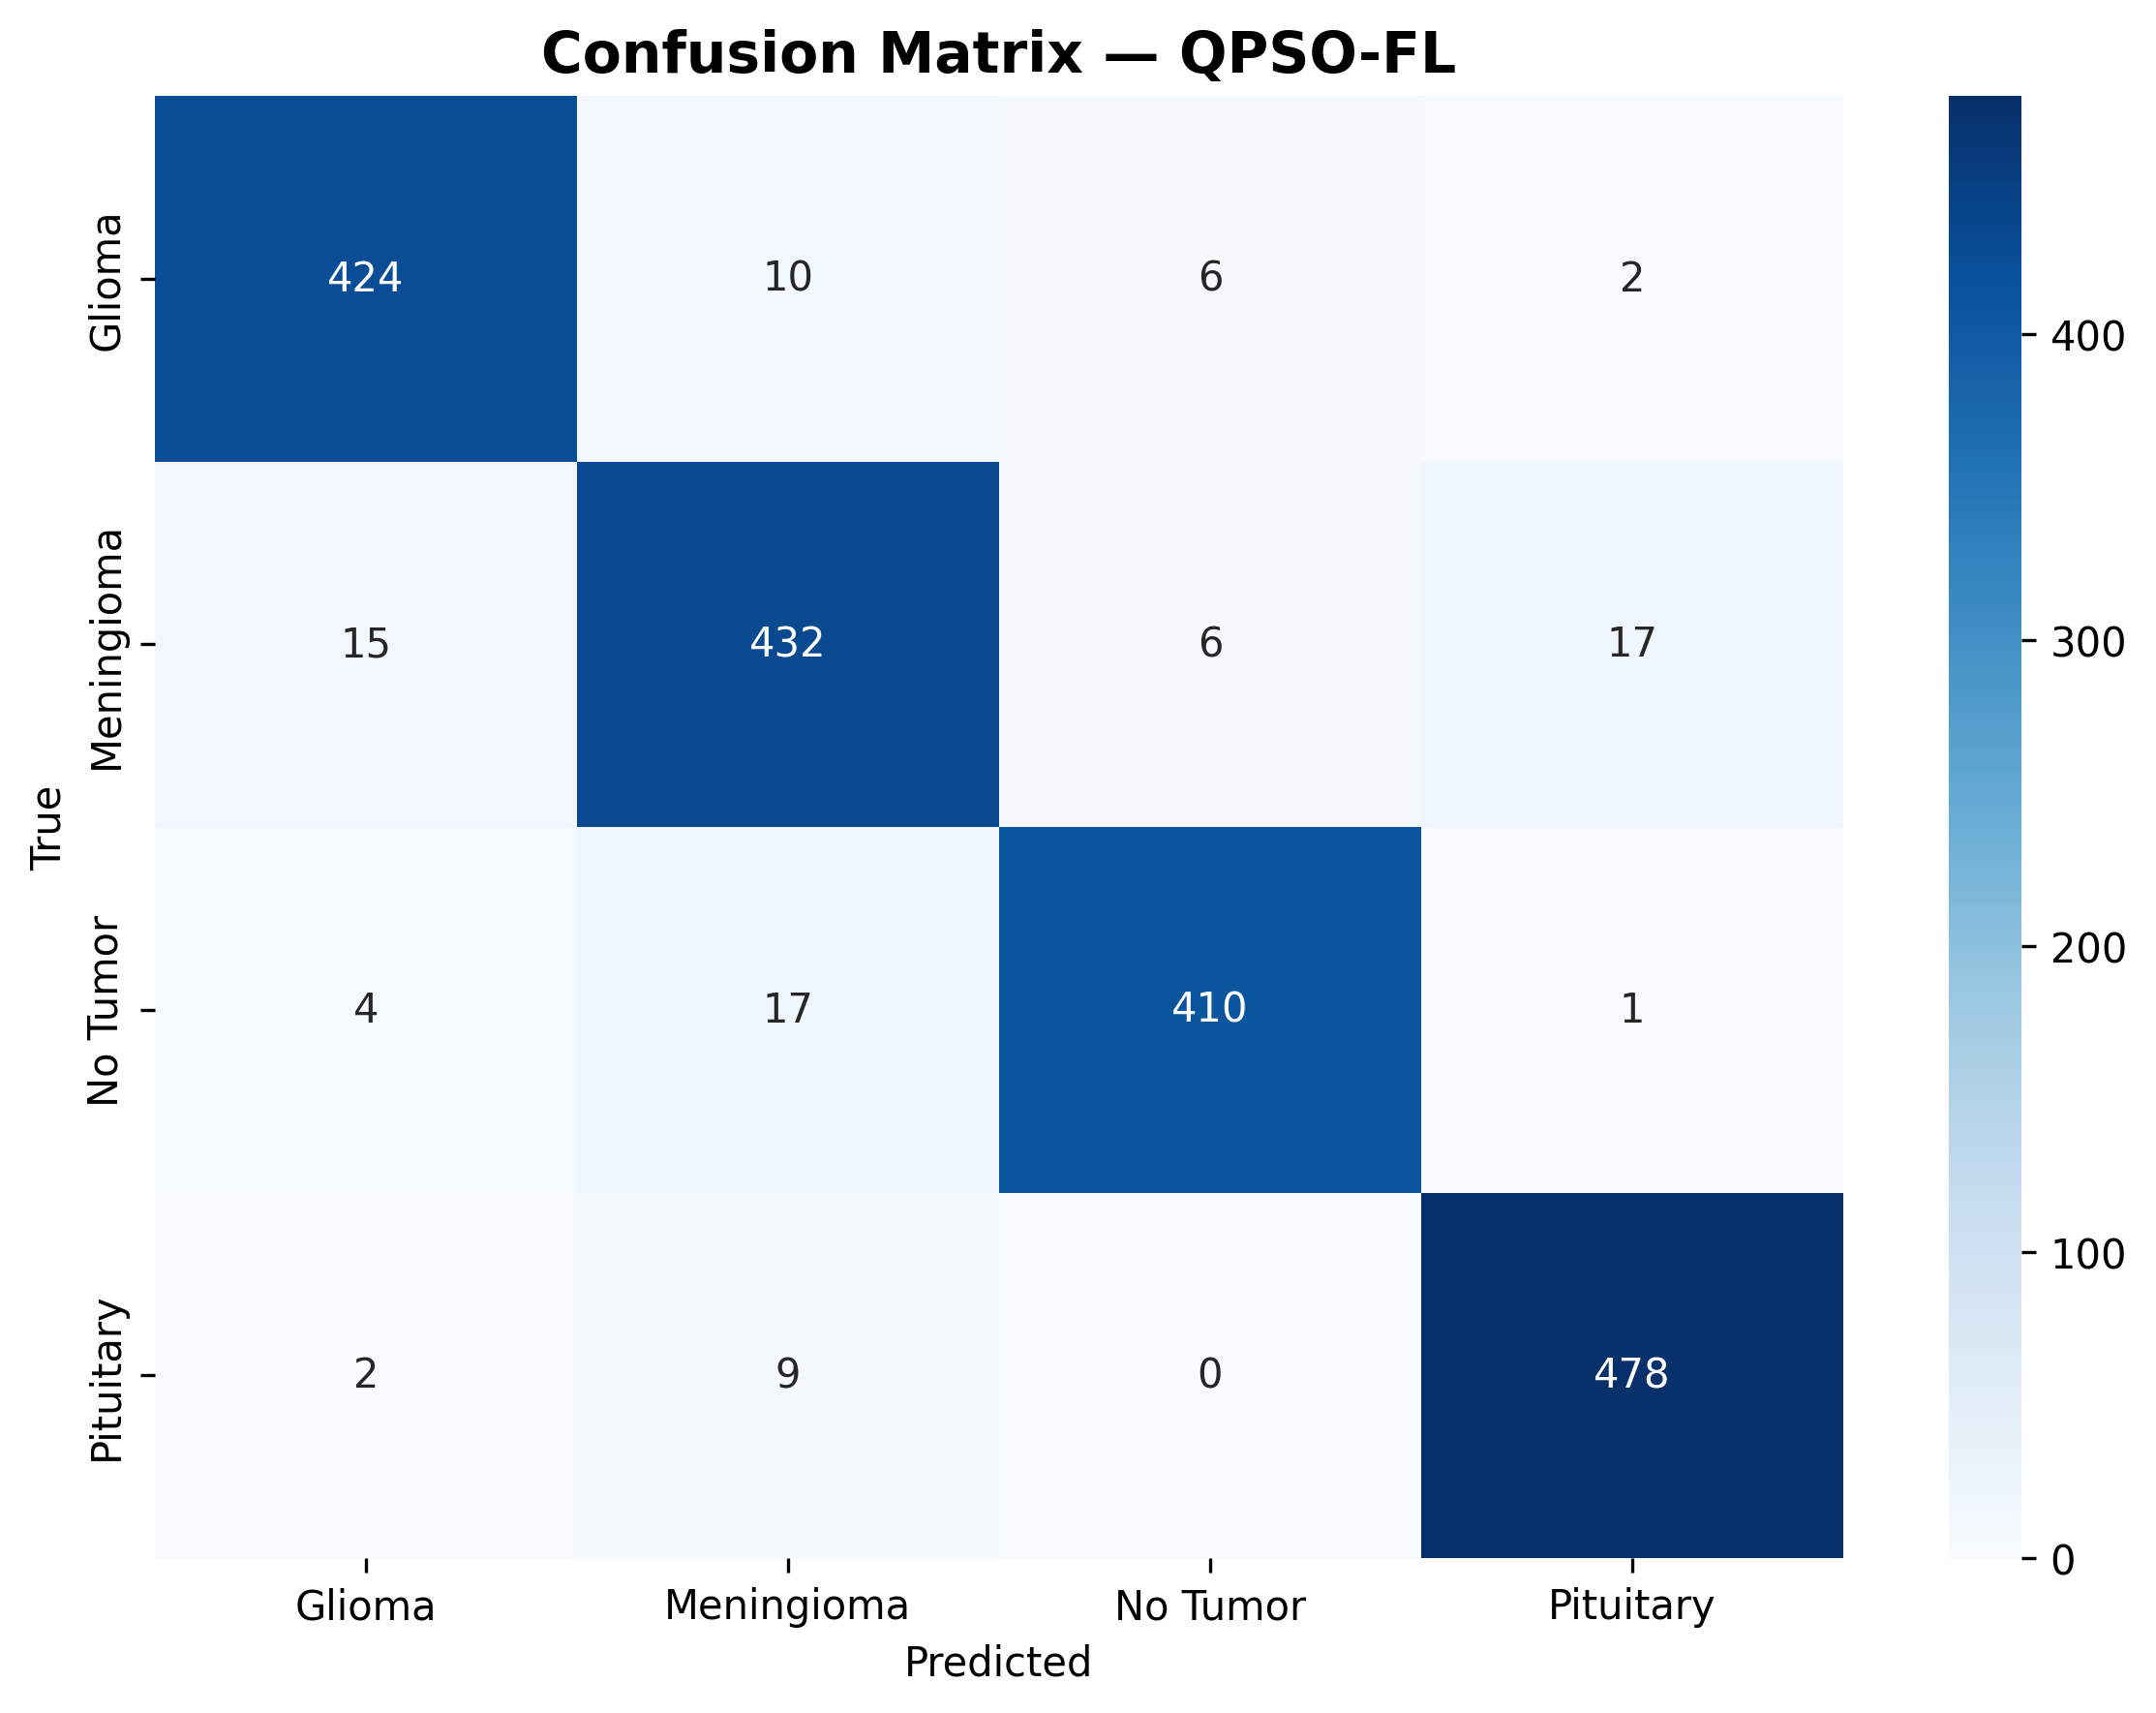
\includegraphics[width=0.32\columnwidth]{s1_cm_qpso.png}}
\caption{Confusion matrices --- Setup~1. Left: FedAvg. Centre: FedProx.
Right: FedQPSO. FedQPSO shows the fewest Glioma misclassifications, with
most off-diagonal errors in the Meningioma class.}
\label{fig:cm_s1}
\end{figure}

\begin{figure}[htbp]
\centerline{%
  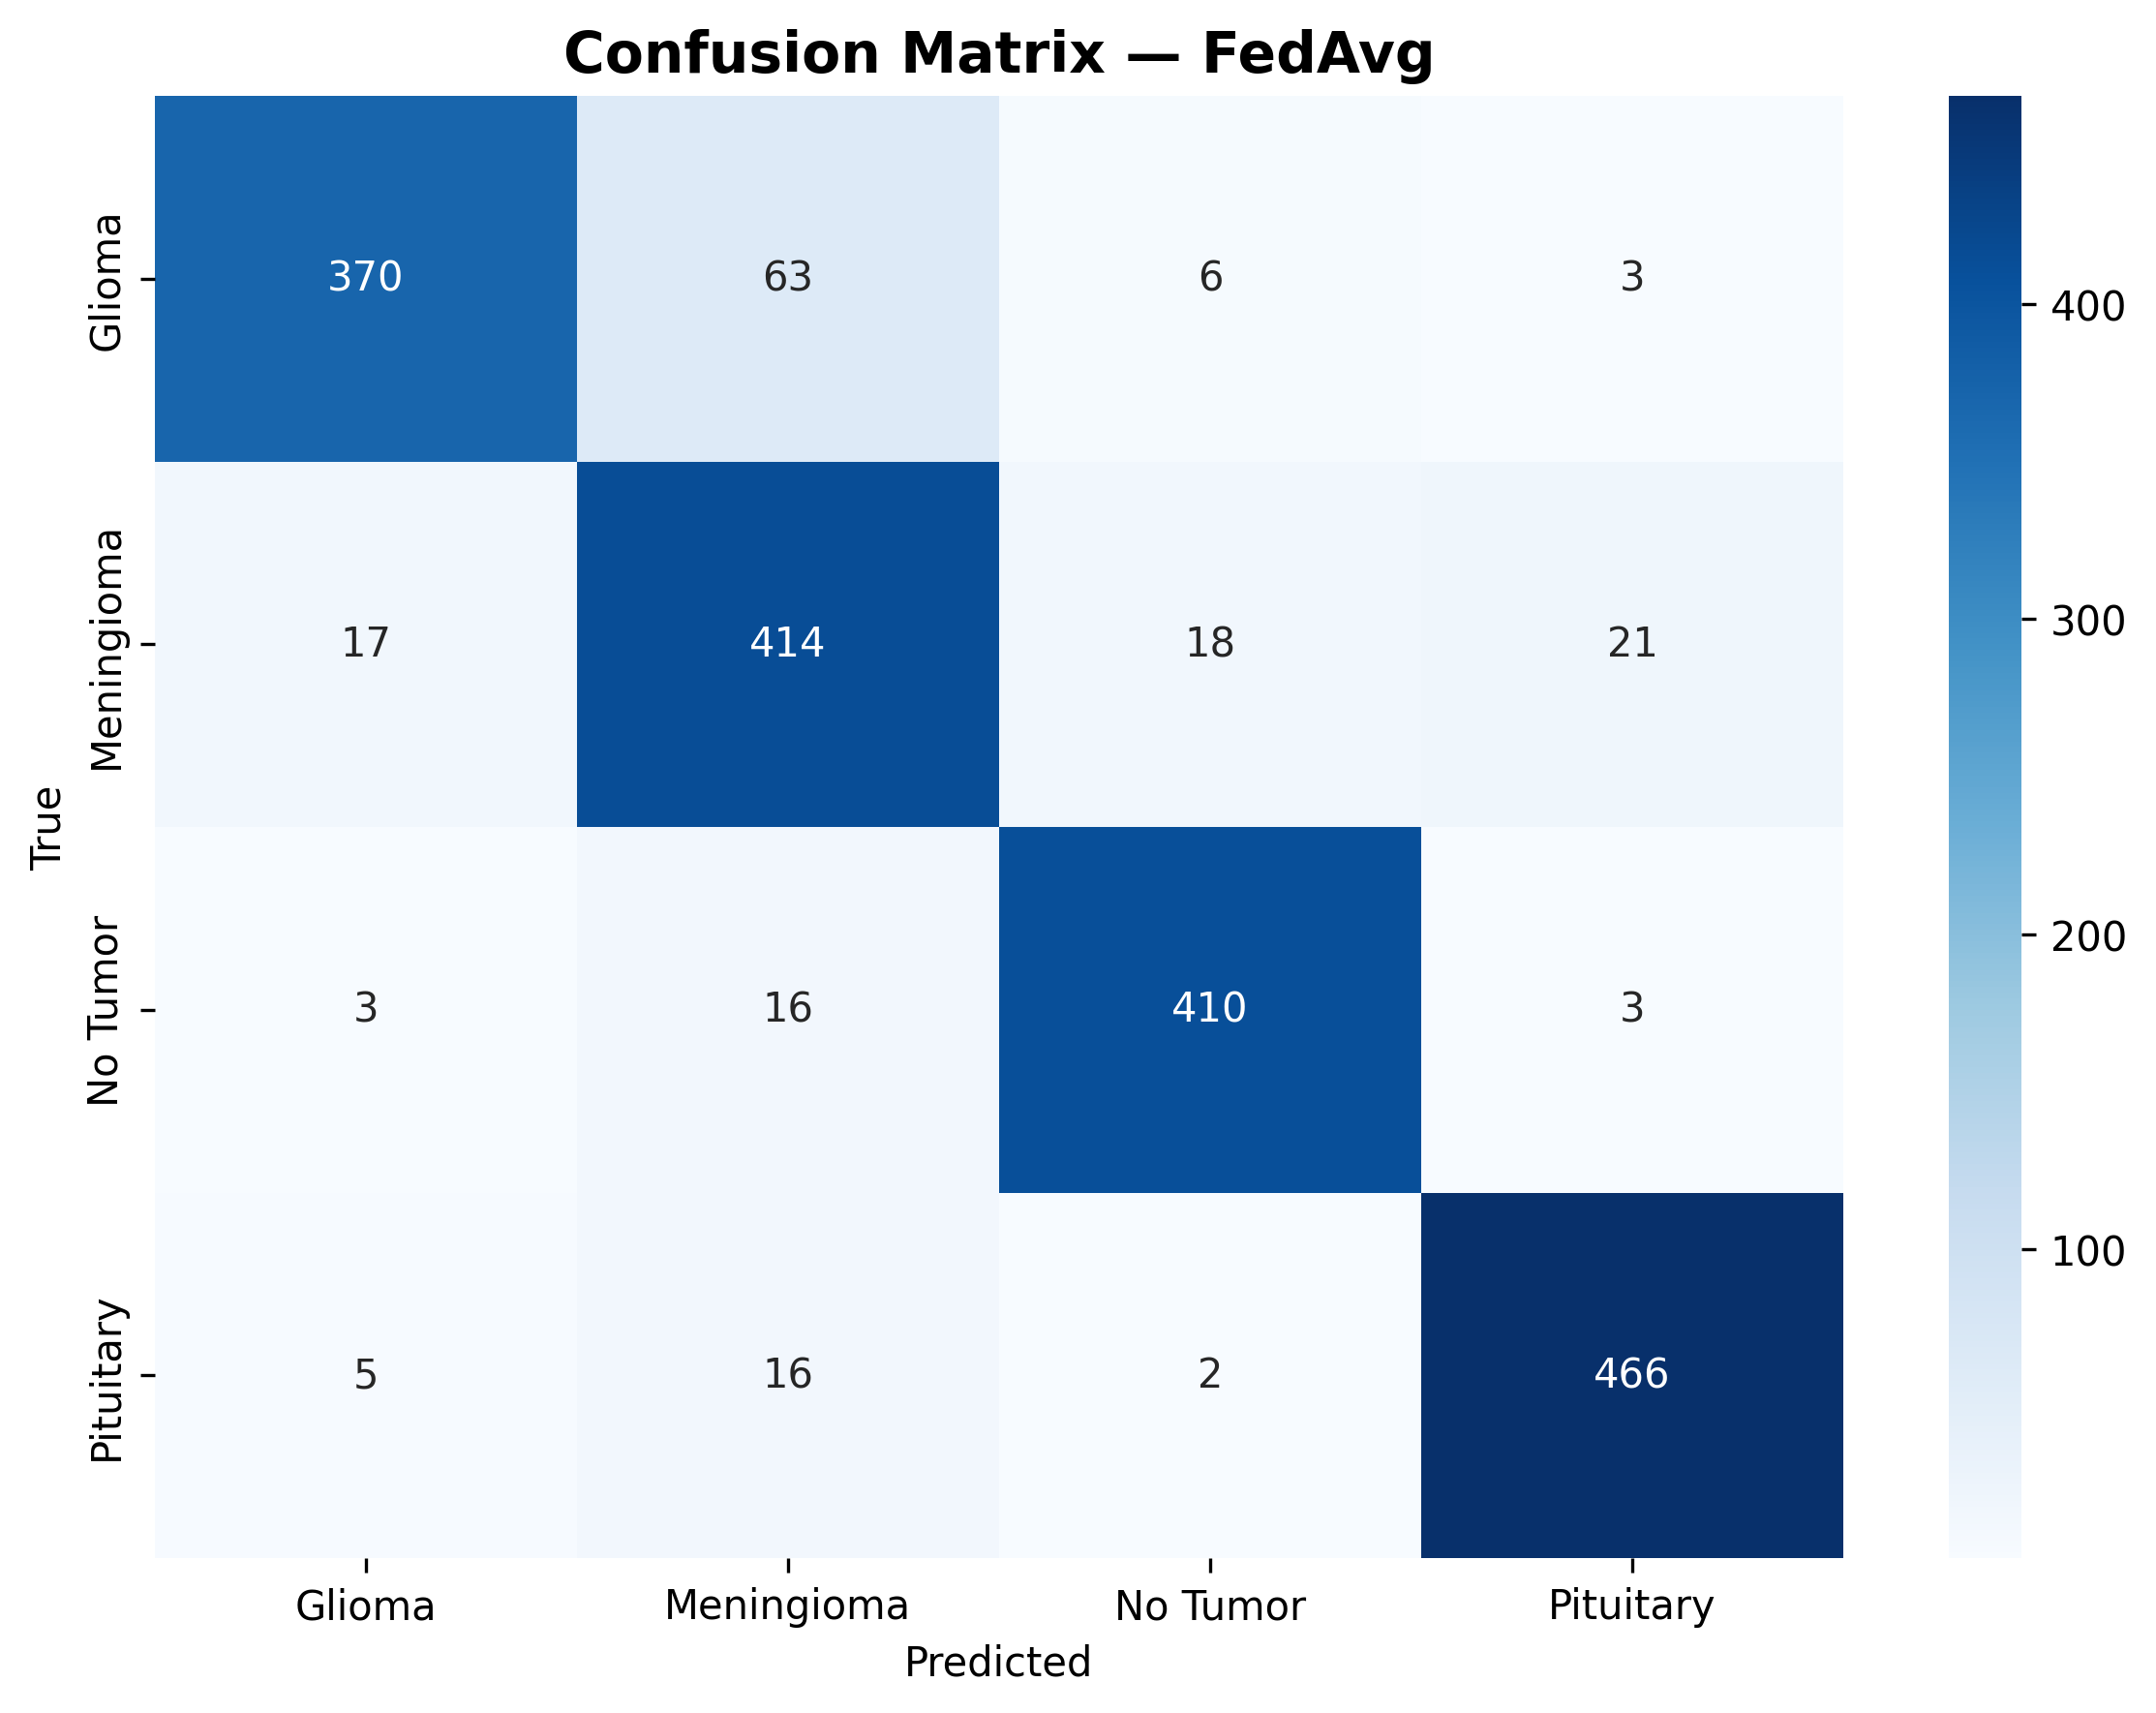
\includegraphics[width=0.32\columnwidth]{s2_cm_fedavg.png}%
  \hfill
  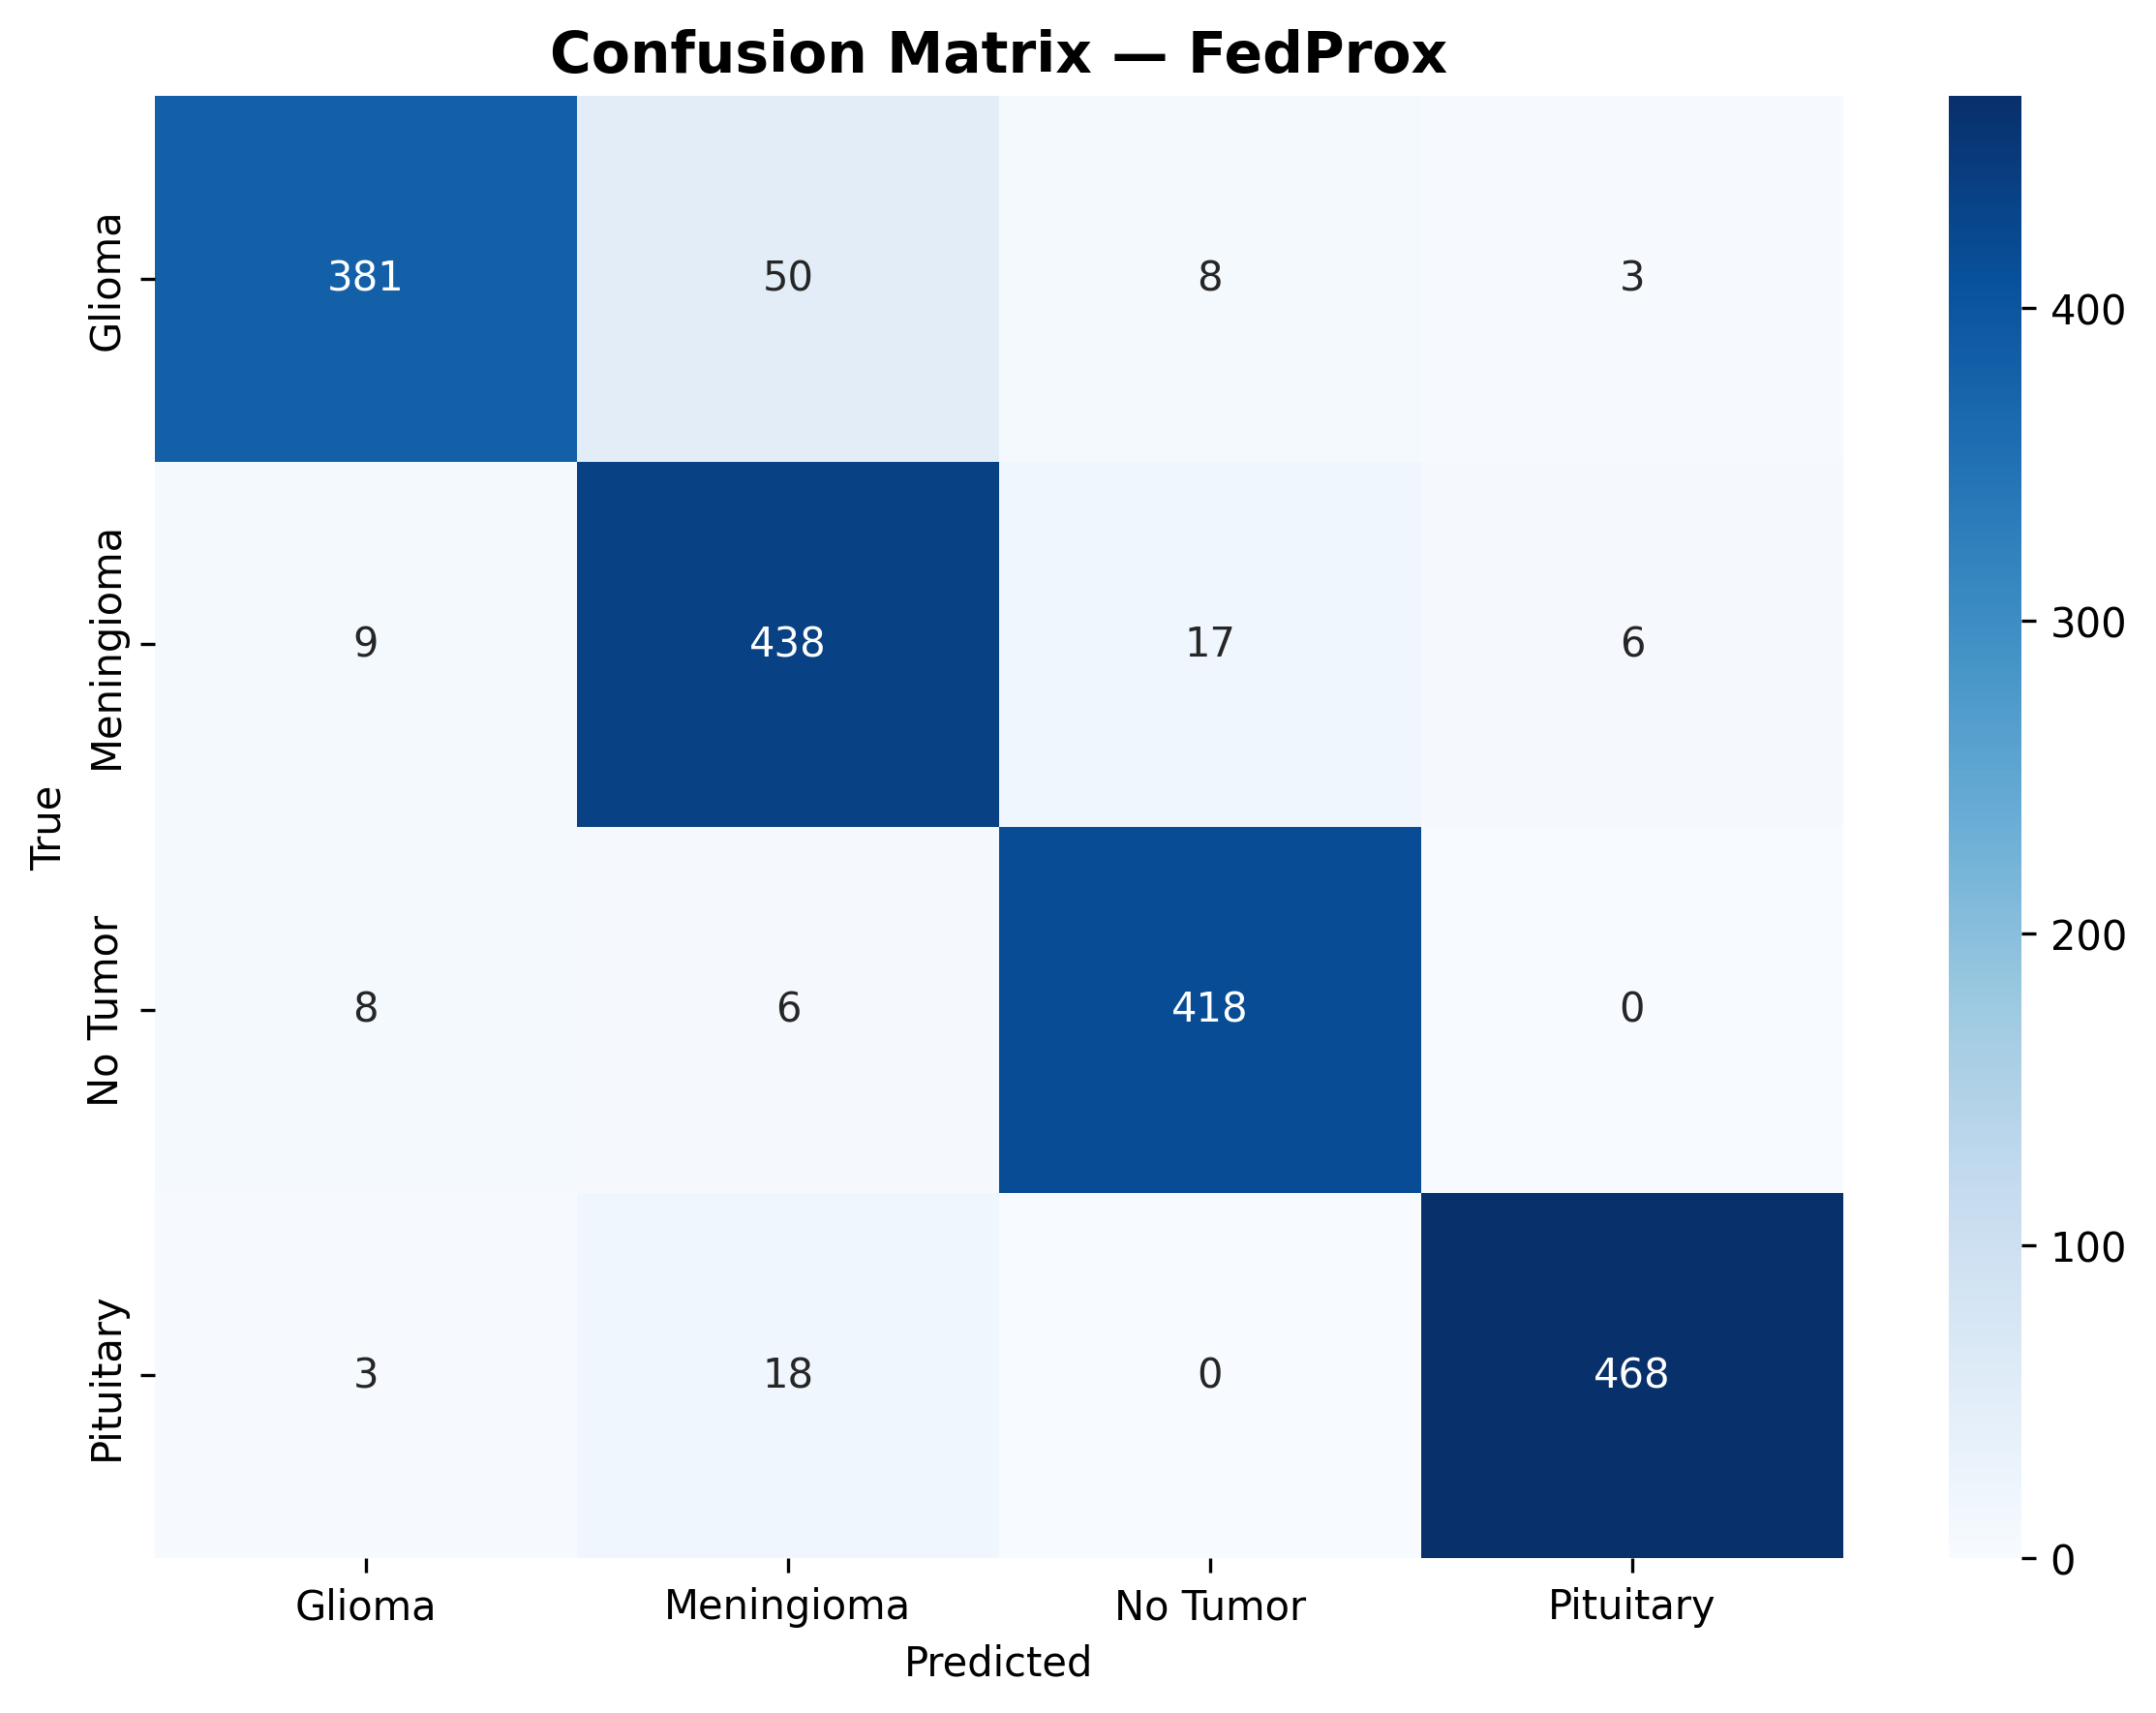
\includegraphics[width=0.32\columnwidth]{s2_cm_fedprox.png}%
  \hfill
  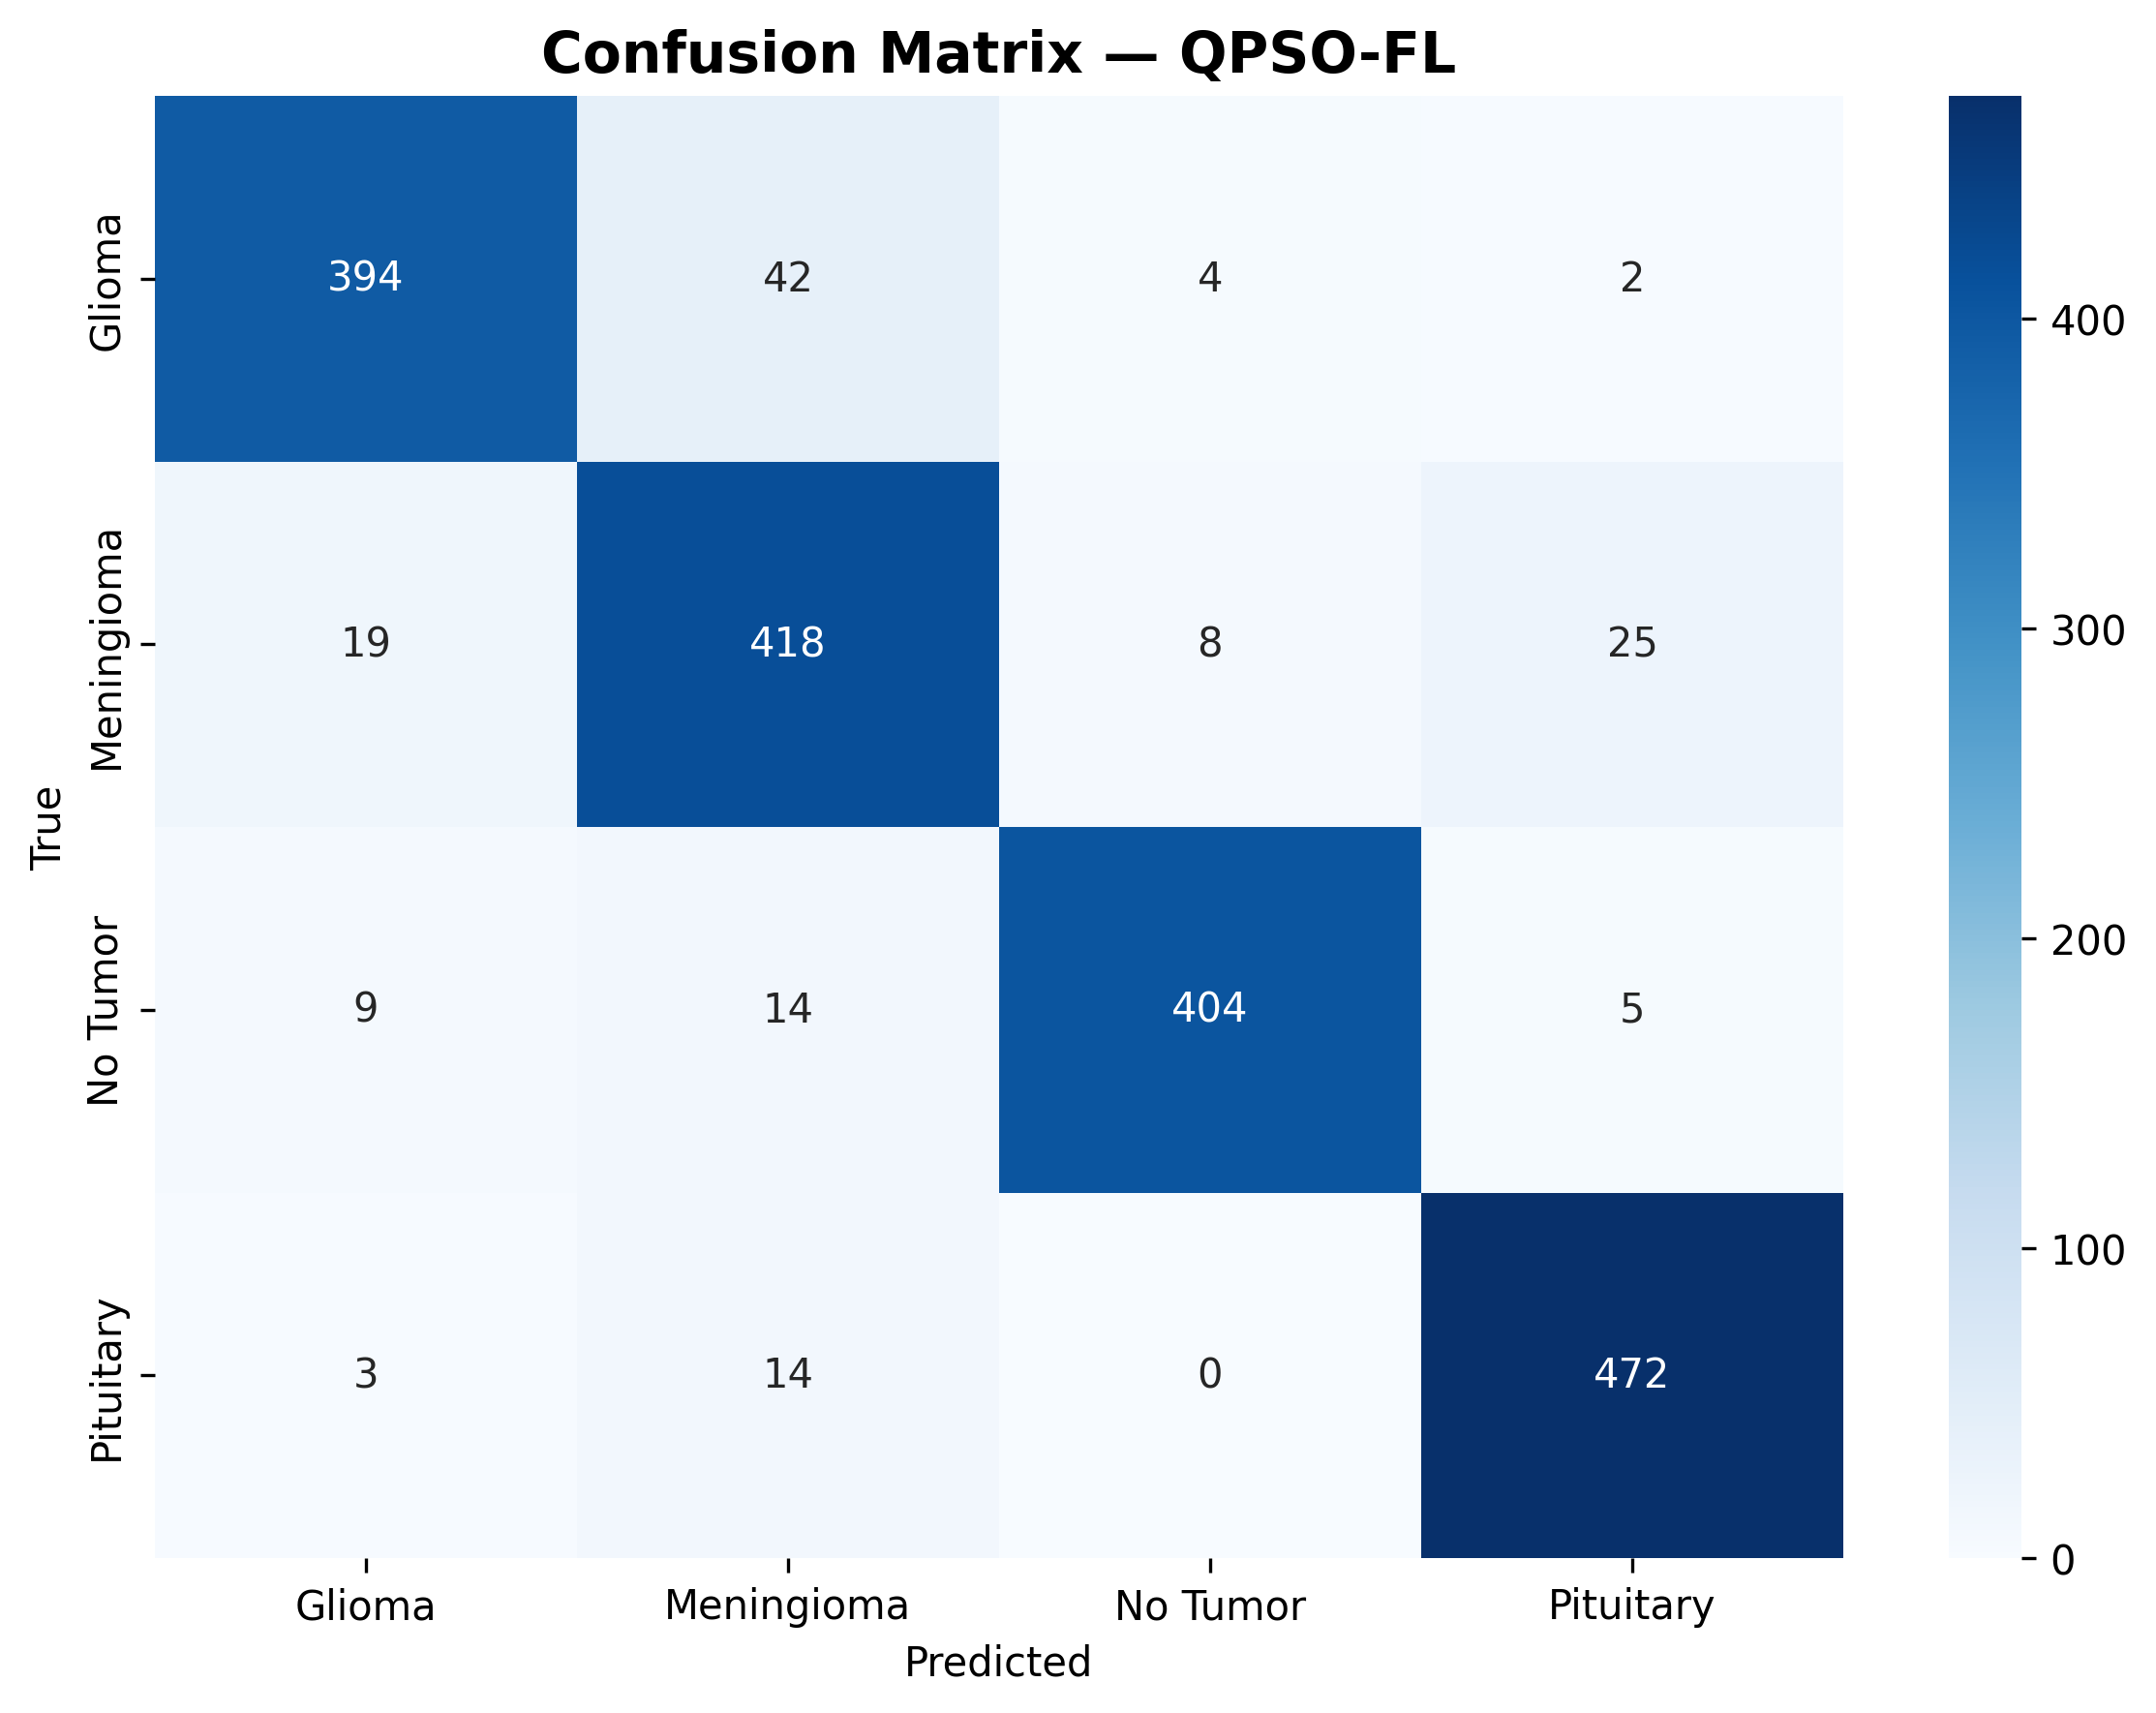
\includegraphics[width=0.32\columnwidth]{s2_cm_qpso.png}}
\caption{Confusion matrices --- Setup~2. Left: FedAvg. Centre: FedProx.
Right: FedQPSO. Under label skew, FedAvg shows pronounced Glioma and
Meningioma confusions driven by per-client distribution bias; FedQPSO and
FedProx exhibit substantially fewer off-diagonal errors.}
\label{fig:cm_s2}
\end{figure}

\subsection{Stability Analysis}

Table~\ref{tab:stability} quantifies accuracy curve volatility.

\begin{table}[htbp]
\caption{Accuracy Curve Stability}
\label{tab:stability}
\begin{center}
\begin{tabular}{llccc}
\hline
\textbf{Setup} & \textbf{Metric} & \textbf{FedAvg} & \textbf{FedProx} &
\textbf{FedQPSO}\\
\hline
\multirow{2}{*}{S1} & Max round drop (pp) & $-$11.51 & $-$8.46 &
\textbf{$-$2.45}\\
 & Round-to-round std (pp) & $\approx$4.0 & $\approx$4.0 & \textbf{2.22}\\
\hline
\multirow{2}{*}{S2} & Max round drop (pp) & $-$14.78 & $-$9.93 &
\textbf{$-$3.38}\\
 & Round-to-round std (pp) & 4.08 & 4.25 & \textbf{2.16}\\
\hline
\end{tabular}
\end{center}
\end{table}

FedQPSO's round-to-round volatility is approximately \textbf{half} that
of both baselines. The largest accuracy drop across FedQPSO's 200 combined
rounds (3.38\,pp, Setup~2) is smaller than FedAvg's single largest crash in
the \emph{easier} natural heterogeneity condition (11.51\,pp). This
stability arises from the fitness evaluation step: unstable weight
combinations are evaluated and rejected before being committed to the global
model, preventing cascading degradation.

% ============================================================
\section{Discussion}
\label{sec:discussion}
% ============================================================

\subsection{Why FedQPSO Is Fairer}
Under FedAvg, Client~3 contributes 3.5$\times$ more samples than Client~1,
giving it proportionally greater influence over every aggregated weight
tensor. FedProx slows all clients equally via the proximal term but does not
redistribute this influence. FedQPSO changes the aggregation objective
entirely: instead of averaging, it searches for the weight configuration
that minimizes loss \emph{jointly across all clients' validation data}. A
solution that achieves low training loss for Clients~2 and~3 but high
validation loss for Client~1 accumulates a high combined fitness score and is
replaced. The implicit fairness constraint emerges naturally from this
structure, with no explicit fairness regularizer or reweighting required.

\subsection{Algorithm Design: Naive vs.\ Layer-by-Layer QPSO}
Early Phase~3 experiments with naive whole-model QPSO --- blind perturbation
of all 120K parameters simultaneously, with no fitness evaluation ---
produced catastrophic results: 77.3\% global accuracy under label skew
versus FedAvg's 90.56\%. The layer-by-layer redesign with validation-loss
fitness evaluation recovered 14.79\,pp and exceeded FedAvg in both setups.
The critical distinction: without evaluating candidate weights, QPSO is
indistinguishable from deliberate noise injection. With per-layer fitness
evaluation, it becomes a disciplined optimization procedure guided by joint
cross-client evidence.

\subsection{Global Accuracy as a Misleading Metric}
At FedAvg's Setup~2 peak (90.56\%), Client~1's concurrent validation
accuracy was 52.92\% --- barely above random chance for a 4-class problem.
At FedQPSO's Setup~2 peak (92.09\%), the same client was at 80.83\%.
Global test accuracy computed on a balanced combined set \emph{actively hides}
severe per-client disparities. In healthcare, this inequity is not a
statistical artifact --- patients at smaller hospitals receive substantially
inferior diagnostic support. We strongly recommend that future FL medical
imaging work always report per-client performance alongside global metrics
(see Table~\ref{tab:fairness}).

\subsection{Clinical Interpretation}
FedQPSO is the \textbf{only} tested algorithm that keeps the weakest client
above 80\% at convergence under label skew. Its superior Glioma recall (0.8914
vs.\ 0.8620 for FedProx and 0.8371 for FedAvg under Setup~2) translates
directly to fewer missed glioma diagnoses. The stability advantage
(max crash $\leq$3.38\,pp vs.\ $\leq$14.78\,pp for FedAvg) is also
clinically meaningful: a sudden 15\,pp degradation during a deployed FL
round would render diagnostic support dangerously unreliable until recovery.

\subsection{Computational Trade-offs}
FedQPSO's 9.4$\times$ compute overhead relative to FedAvg (approximately
125 minutes vs.\ 13 minutes for 100 rounds on a P100 GPU) is its primary
disadvantage. Crucially, this is borne \emph{entirely by the central server}
--- participating hospitals experience identical local training costs.
In offline model development contexts, 2 hours total training is
entirely practical. For high-frequency retraining deployments, the overhead
may be mitigated by reducing $T$, applying FedQPSO only to high-variance
layers, or scheduling QPSO aggregation every $n$ rounds rather than every
round.

% ============================================================
\section{Limitations and Future Work}
\label{sec:limitations}
% ============================================================

\paragraph{Computational cost}
The 9.4$\times$ server overhead limits retraining frequency. Future work
should explore reducing $T$, selective layer application, or periodic QPSO
scheduling to improve wall-clock efficiency.

\paragraph{Client scale}
Only 3 clients were evaluated. Fairness claims should be validated with 5--10
clients simulating more diverse institutional configurations and heterogeneity
profiles.

\paragraph{Architecture}
SimpleCNN was chosen to isolate aggregation as the performance variable.
Evaluating FedQPSO with deeper architectures (EfficientNet-B0, MobileNetV3)
and pretrained models --- with appropriate ablation controls --- would
strengthen generalizability claims.

\paragraph{QPSO hyperparameters}
$\beta = 0.6$ and $T = 5$ were adopted from the MNIST reference
\cite{edla2025mnist} without task-specific tuning. Sensitivity analyses
and adaptive $\beta$ scheduling may improve performance.

\paragraph{Single seed}
Run-to-run variance across multiple random seeds was not measured. Future
work should report mean and confidence intervals over at least 3 independent
runs.

\paragraph{Privacy guarantees}
Only structural privacy via FL is provided. Adding formal differential
privacy (e.g.\ Gaussian gradient noise) may reduce accuracy but would
provide provable privacy bounds alongside FedQPSO's fairness benefits.

% ============================================================
\section{Conclusion}
\label{sec:conclusion}
% ============================================================

We introduced \textbf{FedQPSO}, a novel federated aggregation algorithm
applying layer-by-layer Quantum Particle Swarm Optimization with
validation-loss fitness evaluation to equitable brain tumor MRI classification
across heterogeneous clinical sites. Through a four-phase experimental study
on real-world MRI data, we demonstrated:

\begin{itemize}
    \item FedQPSO reduces the inter-client performance gap by 72--81\%
    compared to FedAvg, and by 45--56\% compared to FedProx.

    \item FedQPSO is the only method maintaining clinically useful
    accuracy ($\geq$80\%) at the weakest client under label skew.

    \item FedQPSO achieves the highest Glioma recall in both conditions
    and the most stable accuracy trajectories (max drop 3.38\,pp vs.\
    14.78\,pp for FedAvg).

    \item FedQPSO's statistical advantage over FedAvg scales with
    heterogeneity severity (Cohen's $d$: $0.35 \to 1.26$), confirming
    the algorithm is most valuable when conditions are most challenging.

    \item The fairness benefit emerges from an implicit mechanism ---
    combined cross-client validation fitness evaluation --- requiring no
    explicit fairness objective or reweighting.
\end{itemize}

These results establish FedQPSO as the preferred aggregation strategy for
fairness-critical federated deployments in multi-institutional medical
imaging where client equity is a primary objective and server-side compute
overhead is acceptable.

% ============================================================
\section*{Acknowledgment}
The authors acknowledge the support of the Department of Computer Science \&
Engineering, Matrusri Engineering College. Compute resources were provided
via Kaggle's GPU platform (Tesla P100-16GB). The Masoud Brain Tumor MRI
dataset and the BRISC 2025 dataset, both publicly available on Kaggle, are
gratefully acknowledged.

% ============================================================
\begin{thebibliography}{00}

\bibitem{mcmahan2017}
H.~B. McMahan, E.~Moore, D.~Ramage, S.~Hampson, and B.~A. y~Arcas,
``Communication-efficient learning of deep networks from decentralized data,''
in \textit{Proc.\ 20th Int.\ Conf.\ Artif.\ Intell.\ Stat.\ (AISTATS)},
Fort Lauderdale, FL, USA, Apr.\ 2017, pp.~1273--1282.

\bibitem{li2020fedprox}
T.~Li, A.~K. Sahu, M.~Zaheer, M.~Sanjabi, A.~Smola, and V.~Smith,
``Federated optimization in heterogeneous networks,''
in \textit{Proc.\ 3rd Conf.\ Mach.\ Learn.\ Syst.\ (MLSys)}, Austin, TX, USA,
Mar.\ 2020, pp.~429--450.

\bibitem{karimireddy2020scaffold}
S.~P. Karimireddy, S.~Kale, M.~Mohri, S.~Reddi, S.~Stich, and A.~T. Suresh,
``SCAFFOLD: Stochastic controlled averaging for federated learning,''
in \textit{Proc.\ 37th Int.\ Conf.\ Mach.\ Learn.\ (ICML)}, Vienna, Austria,
Jul.\ 2020, pp.~5132--5143.

\bibitem{zhao2018}
J.~Zhao, M.~Li, J.~Xu, and W.~Li,
``Federated learning with non-IID data,''
\textit{arXiv:1806.00582}, Jun.\ 2018.

\bibitem{sun2004qpso}
J.~Sun, B.~Feng, and W.~Xu,
``Particle swarm optimization with particles having quantum behavior,''
in \textit{Proc.\ 2004 Congr.\ Evol.\ Comput.\ (CEC)}, Portland, OR, USA,
Jun.\ 2004, vol.~1, pp.~325--331.

\bibitem{sheller2018}
M.~J. Sheller, G.~A. Reina, B.~Edwards, J.~Martin, and S.~Bakas,
``Multi-institutional deep learning modeling without sharing patient data:
A feasibility study on brain tumor segmentation,''
in \textit{Proc.\ Int.\ MICCAI Brainlesion Workshop}, Granada, Spain,
Sep.\ 2018, pp.~92--104.

\bibitem{rieke2020}
N.~Rieke \textit{et al.},
``The future of digital health with federated learning,''
\textit{npj Digit.\ Med.}, vol.~3, no.~1, pp.~1--7, Sep.\ 2020.

\bibitem{sultan2019}
H.~H. Sultan, N.~M. Salem, and W.~Al-Atabany,
``Multi-classification of brain tumor images using deep neural network,''
\textit{IEEE Access}, vol.~7, pp.~69\,215--69\,225, 2019.

\bibitem{ostrom2021}
Q.~T. Ostrom \textit{et al.},
``CBTRUS statistical report: Primary brain and other central nervous system
tumors diagnosed in the United States in 2014--2018,''
\textit{Neuro-oncology}, vol.~23, no.~suppl\_3, pp.~iii1--iii105, 2021.

\bibitem{hipaa}
U.S.\ Department of Health \& Human Services,
``Health Insurance Portability and Accountability Act (HIPAA) of 1996,''
Public Law 104-191, 1996.

\bibitem{kennedy1995}
J.~Kennedy and R.~Eberhart,
``Particle swarm optimization,''
in \textit{Proc.\ ICNN'95 --- Int.\ Conf.\ Neural Netw.}, Perth, WA, Australia,
Nov.--Dec.\ 1995, vol.~4, pp.~1942--1948.

\bibitem{fedpso2021}
J.~Park, H.~J. Kim, and J.~Moon,
``FedPSO: Federated learning using particle swarm optimization to
reduce communication costs,''
\textit{Sensors}, vol.~21, no.~2, p.~600, Jan.\ 2021.

\bibitem{kulkarni2020pfl}
V.~Kulkarni, M.~Kulkarni, and A.~Pant,
``Survey of personalization techniques for federated learning,''
in \textit{Proc.\ 2020 4th World Conf.\ Smart Trends Syst., Secur.\ Sustainability},
London, UK, Jul.\ 2020, pp.~794--797.

\bibitem{masoud}
M. Nickparvar,
``Brain tumor MRI dataset,''
Kaggle, 2021. [Online]. Available:
\url{https://www.kaggle.com/datasets/masoudnickparvar/brain-tumor-mri-dataset}

\bibitem{brisc}
BRISC Dataset Contributors,
``BRISC 2025 brain tumor classification dataset,''
Kaggle, 2025. [Online]. Available:
\url{https://www.kaggle.com/datasets/briscdataset/}

\bibitem{edla2025mnist}
D.~T. Edla,
``Enhancing federated learning with quantum-inspired particle swarm
optimization: An {IID} {MNIST} study,'' (Paper ID: CSE-104)
in \textit{Proc.\ AICTE Sponsored Natl.\ Conf.\ Innovations, Challenges
and Solutions in Eng., Sci.\ and Technol.\ (NCICSET'25)},
Sri Indu College of Engineering and Technology, Hyderabad, India,
Dec.\ 17--18, 2025.

\end{thebibliography}

\end{document}
